%----------Required Packages----------
\documentclass[12pt]{article}
\usepackage[maxauthors=100,articletitle=true]{achemso}
\usepackage[version=4]{mhchem}
\usepackage{geometry}
\usepackage[utf8]{inputenc}
\usepackage{amsmath, amssymb, amsfonts}
\usepackage{siunitx}
\usepackage{multirow}
\usepackage{setspace}
\usepackage{titlesec}
\usepackage{caption}
\usepackage[linktocpage,colorlinks=true,linkcolor=blue,
urlcolor=blue,citecolor=blue,hyperfigures]{hyperref}
\usepackage{graphicx}
\usepackage{float}
\usepackage{setspace}
\usepackage[numbib,nottoc]{tocbibind}
\usepackage{color, colortbl}
\usepackage{enumerate}
\usepackage[table]{xcolor}
\usepackage{tcolorbox}
\usepackage{natbib}
\usepackage{authblk} % For multiple authors and affiliations

%----------Title Section----------
\makeatletter
\renewcommand{\maketitle}{
\begin{center}
{\LARGE \textbf{\@title}} \\[1em]   % Title font size and style
{\large \@author} \\[1em]           % Author font size
{\small \@date}                     % Date font size
\end{center}
}
\makeatother

%----------Useful commands----------
\renewcommand{\arraystretch}{1.5}
\renewcommand\bibname{References}
\setstretch{1.75}

%----------Page layout----------
\geometry{a4paper, margin=1in}
\onehalfspacing

%----------Section formatting----------
\titleformat{\section}{\large\bfseries}{\thesection}{1em}{}
\titleformat{\subsection}{\normalsize\bfseries}{\thesubsection}{1em}{}

%----------Custom Commands----------
\newcommand{\cob}{\color{blue}}
\newcommand{\com}{\color{magenta}}
\newcommand{\voc}{$V_\mathrm{OC}$}
\newcommand{\jsc}{$J_\mathrm{SC}$}
\newcommand{\pce}{PCE$_\mathrm{{max}}$}

\newcommand{\adref}{{\color{magenta}[Reference]}}
\newcommand{\keywords}[1]{\textbf{Keywords:} #1}

%----------Title and Authors----------
\title{Synthesizability-Aware Hybrid Generative Workflow for Donor--Acceptor Discovery in Organic Photovoltaics}

\author[1,*]{Bibhas Das}
\author[1,*]{Anirban Mondal}

\affil[1]{\small Department of Chemistry, Indian Institute of Technology Gandhinagar, Gujarat, 382355, India}

\date{\small\today\\ {E-mail: dasbibhas@iitgn.ac.in, amondal@iitgn.ac.in}}

%----------------------------------------

\begin{document}
\maketitle

\begin{abstract}
Molecular discovery in organic photovoltaics (OPVs) requires simultaneous optimization of donor and acceptor structures, molecular novelty, synthetic practicality, and device-level performance. We present a synthesizability-aware hybrid molecular-generation and screening workflow for OPV donor--acceptor discovery. Twelve complementary proposal and augmentation routes produced class-specific molecular libraries that, after structural validation, canonicalization, deduplication, and adaptive novelty filtering, yielded 52{,}995 unique donor candidates and 53{,}719 unique acceptor candidates with no exact matches to the reference structures. The libraries exhibited substantial scaffold and fingerprint diversity while retaining a measurable relationship to the OPV reference domain. Synthetic practicality was assessed using \texttt{SAScore}, \texttt{RAScore}, and a TANGO-inspired building-block compatibility heuristic; 85.0\% of donors and 99.3\% of acceptors satisfied the operational accessibility screen. Pairing the filtered libraries produced 11{,}988{,}459 donor--acceptor combinations, ranked using a ridge-regression surrogate with isotonic recalibration and Gaussian-process residual correction trained on 300 curated device records. A total of 2{,}832 Tier-2 candidate pairs satisfied joint predicted performance and compatibility criteria, including a small subset with predicted high efficiency and low energy loss. Structure-disjoint validation revealed target-dependent transferability, with particularly limited quantitative reliability for fill factor and open-circuit voltage. The reported device properties are therefore interpreted as screening-based prioritization signals rather than experimentally realized performance. The workflow provides a chemically interpretable route for expanding OPV chemical space and prioritizing donor--acceptor pairs for experimental or higher-fidelity computational follow-up.
\end{abstract}

\section{Introduction}
Organic photovoltaics (OPVs) have emerged as a promising class of solar-energy materials because they combine solution processability, mechanical flexibility, low weight, semi-transparency, and broad chemical tunability. \adref\ \cite{cartlidge2007bright, li2012polymer} These advantages make them attractive for lightweight modules, flexible electronics, building-integrated photovoltaics, and semi-transparent energy-harvesting surfaces \cite{hou2018organic,zhu2024progress}. A major driver of recent progress has been the development of non-fullerene acceptors (NFAs), which have enabled stronger visible-to-near-infrared absorption, tunable frontier orbital energies, reduced voltage losses, and improved donor--acceptor morphology control \cite{hou2018organic,wang2024physical}. As a result, non-fullerene-acceptor-based OPVs have now reached power conversion efficiencies (\pce) exceeding 20\%, establishing them as an important platform for next-generation organic solar-cell (OSC) technologies 
\cite{wang2024physical,zhu2024progress}.

Despite these advances, molecular discovery in OPVs remains intrinsically 
challenging. \cite{wu2020machine} \adref\ Device performance is not determined by a single molecule or a single molecular descriptor, but by the coupled behavior of an electron donor, an electron acceptor, and the nanoscale morphology of their blend. \cite{peng2023materials,wu2020machine} \adref\ The same acceptor can perform differently with different donors, and even the same donor--acceptor pair may exhibit different short-circuit current (\jsc), open-circuit voltage (\voc), fill factor (FF), and \pce\ values depending on energy-level alignment, absorption complementarity, charge-transfer energetics, molecular packing, phase separation, and processing conditions \cite{hou2018organic,zhu2024progress}. OPV materials design is therefore a combinatorial problem in which promising donor and acceptor molecules must be identified together with pairings that satisfy multiple optical, electronic, morphological, and synthetic constraints simultaneously.

Traditional OPV materials discovery has relied on chemical intuition, incremental structural modification, and experimental trial and error. \cite{wu2020machine,peng2023materials} \adref\ Although these approaches have produced many high-performing systems, they are slow compared with the vast chemical space accessible via conjugated polymers and small organic semiconductors. High-throughput virtual screening and machine-learning models have therefore become important tools for accelerating OPV research \cite{miyake2021machine,mahmood2021machine,hachmann2011harvard,wu2020machine}. \adref\ Experimental datasets, such as the OPV database reported by Miyake et al. \cite{miyake2021machine}, provide a useful foundation by linking donor and acceptor structures to device-level properties and molecular descriptors. However, purely predictive models remain limited by the molecules already present in the training data and generally cannot propose new structures outside the explored chemical space.

Generative molecular design offers a complementary strategy by proposing new molecules that satisfy desired property constraints. \cite{sanchezlengeling2018inverse}. \adref\ Variational autoencoders, generative adversarial networks, graph-based generators, reinforcement-learning-guided models, and fragment-based approaches have shown broad potential for molecular design 
\cite{gomezbombarelli2018automatic,guimaraes2017objective,jin2018junction,elton2019deep}. These methods are particularly relevant to OPVs because donor and acceptor molecules can be systematically modified through backbone engineering, side-chain variation, heteroatom substitution, end-group tuning, and fragment recombination. However, molecular generation alone is not sufficient. Generated structures may be chemically invalid, synthetically inaccessible, unstable, too similar to the training set, or irrelevant to OPV chemistry. An effective inverse-design framework must therefore combine molecular generation with chemical validity checks, novelty constraints, synthetic-accessibility assessment, and donor--acceptor-level property evaluation.

Synthetic feasibility is especially important because high predicted performance is not useful if the proposed structures cannot be realistically prepared. Several recent tools address this need. \cite{gao2020synthesizability} \adref\ \texttt{SYBA} estimates whether molecules resemble structures that are likely to be synthetically accessible using a fragment-based Bayesian classifier \cite{vorsilak2020syba}, while \texttt{SCScore} quantifies synthetic complexity from reaction data \cite{coley2018scscore}. Retrosynthesis-aware tools such as \texttt{RAscore} and \texttt{AiZynthFinder} further connect molecular design to plausible synthetic routes and accessible precursors \cite{thakkar2021rascore,genheden2020aizynthfinder}. More recently, \texttt{TANGO} has introduced a constrained synthesizability reward for guiding generative models toward molecules that satisfy property objectives while preserving building-block-level synthetic relationships \cite{guo2026tango}. These developments motivate generative workflows in which synthetic plausibility is treated as an integral component of molecular design rather than as a late-stage post-processing filter.

Here, we present a hybrid molecular-generation and screening workflow for discovering OPV donor and acceptor candidates. The workflow begins with 300 curated donor--acceptor device records derived from our previous work using the experimental OPV resource reported by Miyake \textit{et al.} \cite{miyake2021machine}. These records provide molecular structures and measured device labels for screening-model development. Donors and acceptors are treated as distinct molecular classes throughout standardization, proposal generation, and library-level quality control, and are combined only after molecular filtering. This separation preserves their different electronic roles without relying on unvalidated, hand-coded motif rules.

The framework employs complementary molecular representations: canonical SMILES for sequence-based generation and identity checks; molecular graphs for connectivity-aware generation and validation; three-dimensional coordinates for coordinate-dependent proposal routes; and radius-2, 2048-bit Morgan fingerprints for similarity, novelty, diversity, and pair-level surrogate modeling \cite{rogers2010extended}. Donor and acceptor candidates are proposed through 12 neural, graph-, sequence-, fragment-, template-, mutation-, recombination-, and optimization-guided streams. These streams constitute a hybrid proposal-and-augmentation portfolio rather than 12 independently validated generative models; their outputs are pooled and subjected to a common standardization and filtering procedure, combining data-driven generation with chemically interpretable local exploration of the reference chemical space.

Each proposed molecule is canonicalized and re-parsed before screening. Retained candidates must form valid, single-component, non-radical molecular graphs; be absent from the training library; be unique within the generated library; and satisfy an adaptive Morgan--Tanimoto nearest-neighbor novelty criterion. Synthetic practicality is treated as a prioritization attribute rather than as evidence of a confirmed route, assessed using fragment-based synthetic-accessibility scoring, a retrosynthetic-accessibility classifier, and a \texttt{TANGO}-inspired building-block-compatibility heuristic. Filtered donors and acceptors are then paired and evaluated using fingerprint- and descriptor-based surrogates for \pce, \jsc, \voc, and FF, together with an energy-loss quality-control screen.

This workflow addresses three principal OPV-discovery challenges: expanding donor and acceptor chemical space beyond top-down screening; reducing invalid, redundant, and synthetically impractical candidates through explicit chemical-quality and novelty controls; and evaluating performance at the donor--acceptor-pair level. Device-property estimates are used for target-dependent ranking and prioritization, with structure-disjoint validation defining their limitations; they are not interpreted as experimentally realized performance. Overall, the framework provides a practical route for identifying chemically plausible OPV candidates for subsequent experimental or higher-fidelity computational assessment.

\section{Computational Methods}

\subsection{Study Design and Computational Workflow}
We developed a distributed, hybrid molecular-design workflow to propose and prioritize OPV donor and NFA candidates. The workflow was structured as a sequence of chemically conservative decision stages rather than as a single end-to-end predictor: (i) curation and standardization of experimentally characterized donor--acceptor pairs; (ii) class-specific molecular representation and proposal generation; (iii) molecular validity, uniqueness, and novelty control; (iv) synthetic-accessibility and building-block compatibility ranking; and (v) paired donor--acceptor property prediction and multi-property prioritization. Donors and acceptors were maintained as separate chemical populations throughout standardization, generation, and library-level quality control, and were combined only after the molecular filters had been applied and the paired device properties had been evaluated.

The generative component was deliberately treated as a chemical-space expansion tool, not as evidence that a generated molecule is synthesizable or that a predicted device efficiency will be experimentally realized. Likewise, the screening models were used to rank candidates for subsequent experimental or higher-fidelity computational assessment rather than to make claims of experimentally validated device performance. This separation of generation, chemical quality control, and property ranking reduces the risk that a candidate is retained solely based on an extrapolative model prediction. The workflow combined trainable molecular proposal models with deterministic and fragment-guided proposal routes, an important design choice given that the 
available paired OPV training data are modest relative to the breadth of chemically accessible donor and acceptor space. All proposals, regardless of their origin, entered a common canonicalization and filtering procedure before any library-level statistics or device-property estimates were calculated.

\subsection{Dataset Preparation and Molecular Standardization}
The starting point was a curated paired-device library constructed in our previous work from the experimental OPV resource reported by Miyake \textit{et al.} \cite{miyake2021machine}. The source contains 1318 reported devices, 667 acceptors, and 279 donors; these values reflect the larger literature-derived source database, not the final analysis subset used here. The present study used a curated subset of 300 donor--acceptor device records, which contains 299 acceptor entries and 38 donor entries at the level of the unstandardized structural strings. Each record provides a donor structure, an acceptor structure, and the measured device labels used for model development: \jsc, \voc, FF, and \pce. The curated table also retains device energy-loss information for the separate energy-loss quality-control analysis. This 300-record subset was used because it already carries the validated, consistent DFT/TD-DFT descriptor annotation required for both device-performance modeling and energy-loss screening \cite{das2024predictive}. Extending these calculations to the full Miyake resource would require quantum-chemical annotation of several hundred additional unique donor and acceptor structures and was beyond the scope of this study.

The use of a paired-device subset has an important consequence: the 300 records are device observations, not 300 mutually independent NFAs. Accordingly, all reported performance estimates and chemical-space analyses distinguish between a molecular library and the donor--acceptor device records from which the paired regression targets were learned. Records with incomplete labels for a given device target were excluded only from the corresponding target-specific model-development subset; the four principal device labels in the curated 300-record table were complete.

Molecular parsing, sanitization, canonicalization, substructure analysis, and fingerprint calculation were performed with RDKit \cite{landrum2013rdkit}. Every molecular string was converted into a sanitized molecular graph before being admitted to the curated training population or the generated candidate pool. Canonical structural strings were then used as molecular identifiers for duplicate detection and train--generated overlap checks, thereby avoiding the treatment of alternative string encodings of the same molecular graph as distinct molecules. Molecular structures that could not be parsed and sanitized, that contained disconnected components, or that represented radicals were excluded from the final candidate libraries. No arbitrary structural rewriting was used to convert an invalid generated string into a different molecule. When a coordinate-based proposal route was used, conformers were first embedded and relaxed with molecular mechanics routines; a structure that failed to generate coordinates was unavailable to that particular route but could still be represented by its sanitized molecular graph for the remaining compatible stages. Failed conformer generation was therefore not conflated with chemical invalidity.

\subsection{Molecular Representations}
Different representations were used for complementary tasks. Canonical SMILES strings provided a compact representation for sequence-oriented proposal routes and exact-identity checks. Molecular graphs preserved atom types, bond types, and connectivity for graph-oriented operations and chemical validation. Three-dimensional coordinates were used only by coordinate-dependent proposal modules. Circular Morgan fingerprints (radius 2; 2048 bits) were used for train--generated similarity calculations, diversity analysis, building-block comparison, and donor--acceptor pair regression \cite{rogers2010extended}. This fingerprint specification was held constant across the nearest-neighbor, internal-diversity, and molecular-library quality analyses. Morgan fingerprints 
are well suited to this workflow because they encode local chemical environments in a fixed-length representation while supporting direct Tanimoto-similarity comparisons.

For sequence modules requiring a grammar-constrained string alphabet, a SELFIES-compatible representation could be used as a fallback to reduce invalid-string production \cite{krenn2020self}. This fallback did not bypass the final RDKit validation step: every proposed structure, irrespective of its internal representation, was required to yield a valid, canonical molecular graph before further processing. The use of multiple representations was therefore functional rather than redundant, with each addressing a distinct part of the proposal, validation, or ranking problem.

\subsection{Hybrid Molecular Generation}
Candidate donors and acceptors were proposed independently using a hybrid generation strategy. The 12-route portfolio included character- and graph-based generative adversarial approaches; conditional and multi-objective variants; active- and reinforcement-learning-guided proposal routes; transformer- and junction-tree-based generation; a variational autoencoder; graph-constrained generation; transfer-learning-based variation; and training-set-anchored augmentation. These routes were executed as separate proposal streams and pooled before common molecular standardization. Their designation as distinct computational routes does not imply that every stream represents an independently validated generative model. The donor coordinate-based GAN was trained on 299 valid coordinate instances, although these represent only 38 unique donor chemotypes; repeated device records, therefore, increase the number of conformational instances but not donor-side structural diversity. The coordinate GAN was consequently only one component of the 12-route proposal framework. All candidates underwent exact-identity and near-neighbor novelty filtering (Section~2.5); the retained donor library had a mean nearest-neighbor Tanimoto similarity of $0.171$, with $97.0\%$ of structures below $0.5$. These results are inconsistent with a library dominated by training-set replicas, but they do not establish broad donor-side generalization, which is assessed separately through structure-disjoint validation.

The nominal number of proposal branches should not be interpreted as the number of independently validated generative models. Several branches are deterministic or semi-deterministic expansion procedures, and their availability depends on the molecules, fragments, and valid intermediate structures obtained for a given class. Fragment, scaffold, mutation, recombination, and backfill operations provide chemically interpretable methods for expanding sparse proposal streams. When a route generated too few viable candidates, structurally controlled SMARTS-based transformations, BRICS-compatible recombination, and related graph or fragment variants were used to increase candidate coverage. Training structures were permitted to serve as chemically meaningful starting points for controlled variation but were not retained automatically as generated discoveries. Each resulting proposal underwent the same canonicalization, exact-novelty, duplicate-removal, and similarity-novelty procedures described in Section~2.5. Full details of neural component implementation, adversarial training monitoring, convergence criteria, and hyperparameter optimization are provided in the Supporting Information.

\subsection{Chemical Validity and Novelty Filtering}
All proposed molecules were processed through a common acceptance pipeline. A candidate was retained only if it produced a sanitized canonical RDKit molecule, consisted of a single non-radical component, was absent from the corresponding training set, and was not a duplicate of an already accepted generated molecule. The order of these checks was fixed to ensure that validity and identity were assessed before similarity-based novelty. Exact novelty was determined from canonical structures, whereas near-neighbor novelty was determined from Morgan-fingerprint similarity.

For two molecular fingerprints $A$ and $B$, Tanimoto similarity was calculated as
\begin{equation}
T(A,B)=\frac{|A\cap B|}{|A|+|B|-|A\cap B|}.
\end{equation}
For a candidate $m$, the relevant similarity statistic was the maximum similarity to any molecular structure in the corresponding donor or acceptor training population,
\begin{equation}
S_{\max}(m)=\max_{r\in\mathcal{R}} T(m,r),
\end{equation}
where $\mathcal{R}$ denotes the relevant reference set. A size-adaptive cutoff was used because an identical fixed similarity criterion can be disproportionately permissive for large conjugated structures and disproportionately restrictive for smaller molecules. With $N_{\mathrm{HA}}$ denoting the heavy-atom count, the threshold was defined as
\begin{equation}
\tau(N_{\mathrm{HA}})=
\begin{cases}
0.40, & N_{\mathrm{HA}}\leq 30,\\
0.40+\dfrac{(0.75-0.40)(N_{\mathrm{HA}}-30)}{150-30}, 
  & 30<N_{\mathrm{HA}}<150,\\
0.75, & N_{\mathrm{HA}}\geq 150.
\end{cases}
\end{equation}
A candidate was retained only when $S_{\max}(m)<\tau(N_{\mathrm{HA}})$. This adaptive rule preserves a consistent interpretation of novelty across the broad molecular-size range encountered in the generated libraries.

The post-generation gate was intentionally limited to defensible 
chemical-validity, identity, and similarity criteria. It did not treat a hand-coded donor or acceptor motif rule, a narrow molecular-size window, or an unvalidated physicochemical cutoff as proof of OPV relevance. Such rules can remove genuinely useful chemotypes and encode historical design bias. OPV relevance was instead addressed downstream through paired property ranking and through transparent synthetic-accessibility and building-block-compatibility indicators, making the separation between chemical validity, structural novelty, 
synthetic practicality, and predicted device performance explicit.

\subsection{Synthesizability Assessment}
Synthetic practicality was evaluated as a ranking problem rather than as a binary claim of route availability. Each retained molecule was first assigned a synthetic-accessibility score using the established fragment-based \texttt{SAScore} formulation implemented within the RDKit contribution framework \cite{sascore}. This score summarizes the prevalence of molecular fragments and structural complexity and was used to distinguish relatively accessible candidates from structurally demanding ones within the generated library. It was not interpreted as a guarantee of calculated synthetic yield, cost, or experimental feasibility.

For operational library triage, candidates satisfying \texttt{SAScore} $\leq 6.0$ and a retrosynthetic-accessibility score $\geq 0.5$ were labeled synthetically promising. These thresholds define a screening subset; they do not remove molecules from the chemically valid parent library nor establish the existence of an experimental synthesis route. A TANGO-inspired building-block compatibility indicator was additionally calculated from fuzzy substructure overlap and fingerprint similarity to OPV-relevant building blocks and BRICS-derived fragments represented in the curated chemistry. The score was defined as
\begin{equation}
S=\alpha\,\mathrm{FMS}+(1-\alpha)\,\mathrm{BB\text{-}Tanimoto},
\end{equation}
where $\mathrm{FMS}$ is the fragment-match component, 
$\mathrm{BB\text{-}Tanimoto}$ quantifies overlap with the reference 
building-block collection, and $\alpha=0.5$. The term ``TANGO-inspired'' is used deliberately: the indicator serves as a domain-specific compatibility heuristic and is not presented as a reproduction of the published TANGO methodology or as a universal measure of synthetic accessibility \cite{tango}. Candidates with favorable fragment compatibility and acceptable synthetic-accessibility scores were prioritized for inspection, while the complete score distribution was 
retained to avoid concealing trade-offs between structural novelty and practical complexity.

Classifier-style retrosynthetic scores, including \texttt{RAScore}-like assessments, are useful for triaging large libraries but do not, by themselves, establish the existence of a complete, purchasable, and chemically plausible route \cite{rascore}. Accordingly, a route-findability label produced with this backend was reported as a model classification rather than as a confirmed route. Formal route confirmation requires an independently documented retrosynthetic search and examination of the proposed precursors and transformations; tools such as \texttt{AiZynthFinder} provide one possible framework for that separate validation step \cite{genheden2020aizynthfinder}.

\subsection{Donor--Acceptor Pair Construction and Property Prediction}
Only donors and acceptors passing the molecular-level filters entered the pair-evaluation stage. Candidate pairing was managed to preserve the representation of distinct structural and predicted-property regimes when the full donor--acceptor Cartesian product was computationally impractical. This trait-balanced pairing strategy directs screening toward chemically diverse combinations rather than repeatedly evaluating closely related structures.

Paired device-property models were developed from the curated experimental device records. For each pair, the donor and acceptor fingerprint vectors were concatenated to explicitly encode both members of the heterojunction. The screening representation also incorporated the available molecular descriptors for the paired components. Separate regressors were developed for \jsc, \voc, FF, and \pce, with candidate model families compared by held-out performance for each response rather than assuming that one modeling architecture is uniformly optimal. The final pair-level screening surrogate used ridge regression with isotonic recalibration and a Gaussian-process residual correction, providing a consistent ranking representation for the combined donor--acceptor space. These predictions are screening estimates and are not a direct substitute for experimental device measurements.

Predictive reliability was evaluated using complementary structure-disjoint protocols. Donor-disjoint, acceptor-disjoint, and Bemis--Murcko scaffold-disjoint splits were used for diagnostic evaluation of the molecular and device-property models, whereas donor-group-disjoint cross-validation was used for the paired-screening workflow. In the latter protocol, all records associated with a given donor identity were assigned to the same validation fold, so that each validation prediction was made for a donor not present in the corresponding training fold. The validation procedures, therefore, test transferability across explicitly withheld molecular structures but do not constitute experimental device validation. Predictive performance was summarized using standard out-of-fold regression statistics, including root-mean-square error, mean absolute error, coefficient of determination, and the correlation between observed and predicted values. Classical regression, Gaussian process modeling, dimensionality reduction, and statistical metrics were implemented using scikit-learn \cite{pedregosa2011scikit}; numerical operations were performed using SciPy \cite{virtanen2020scipy}.

\begin{figure}[!htb]
\centering
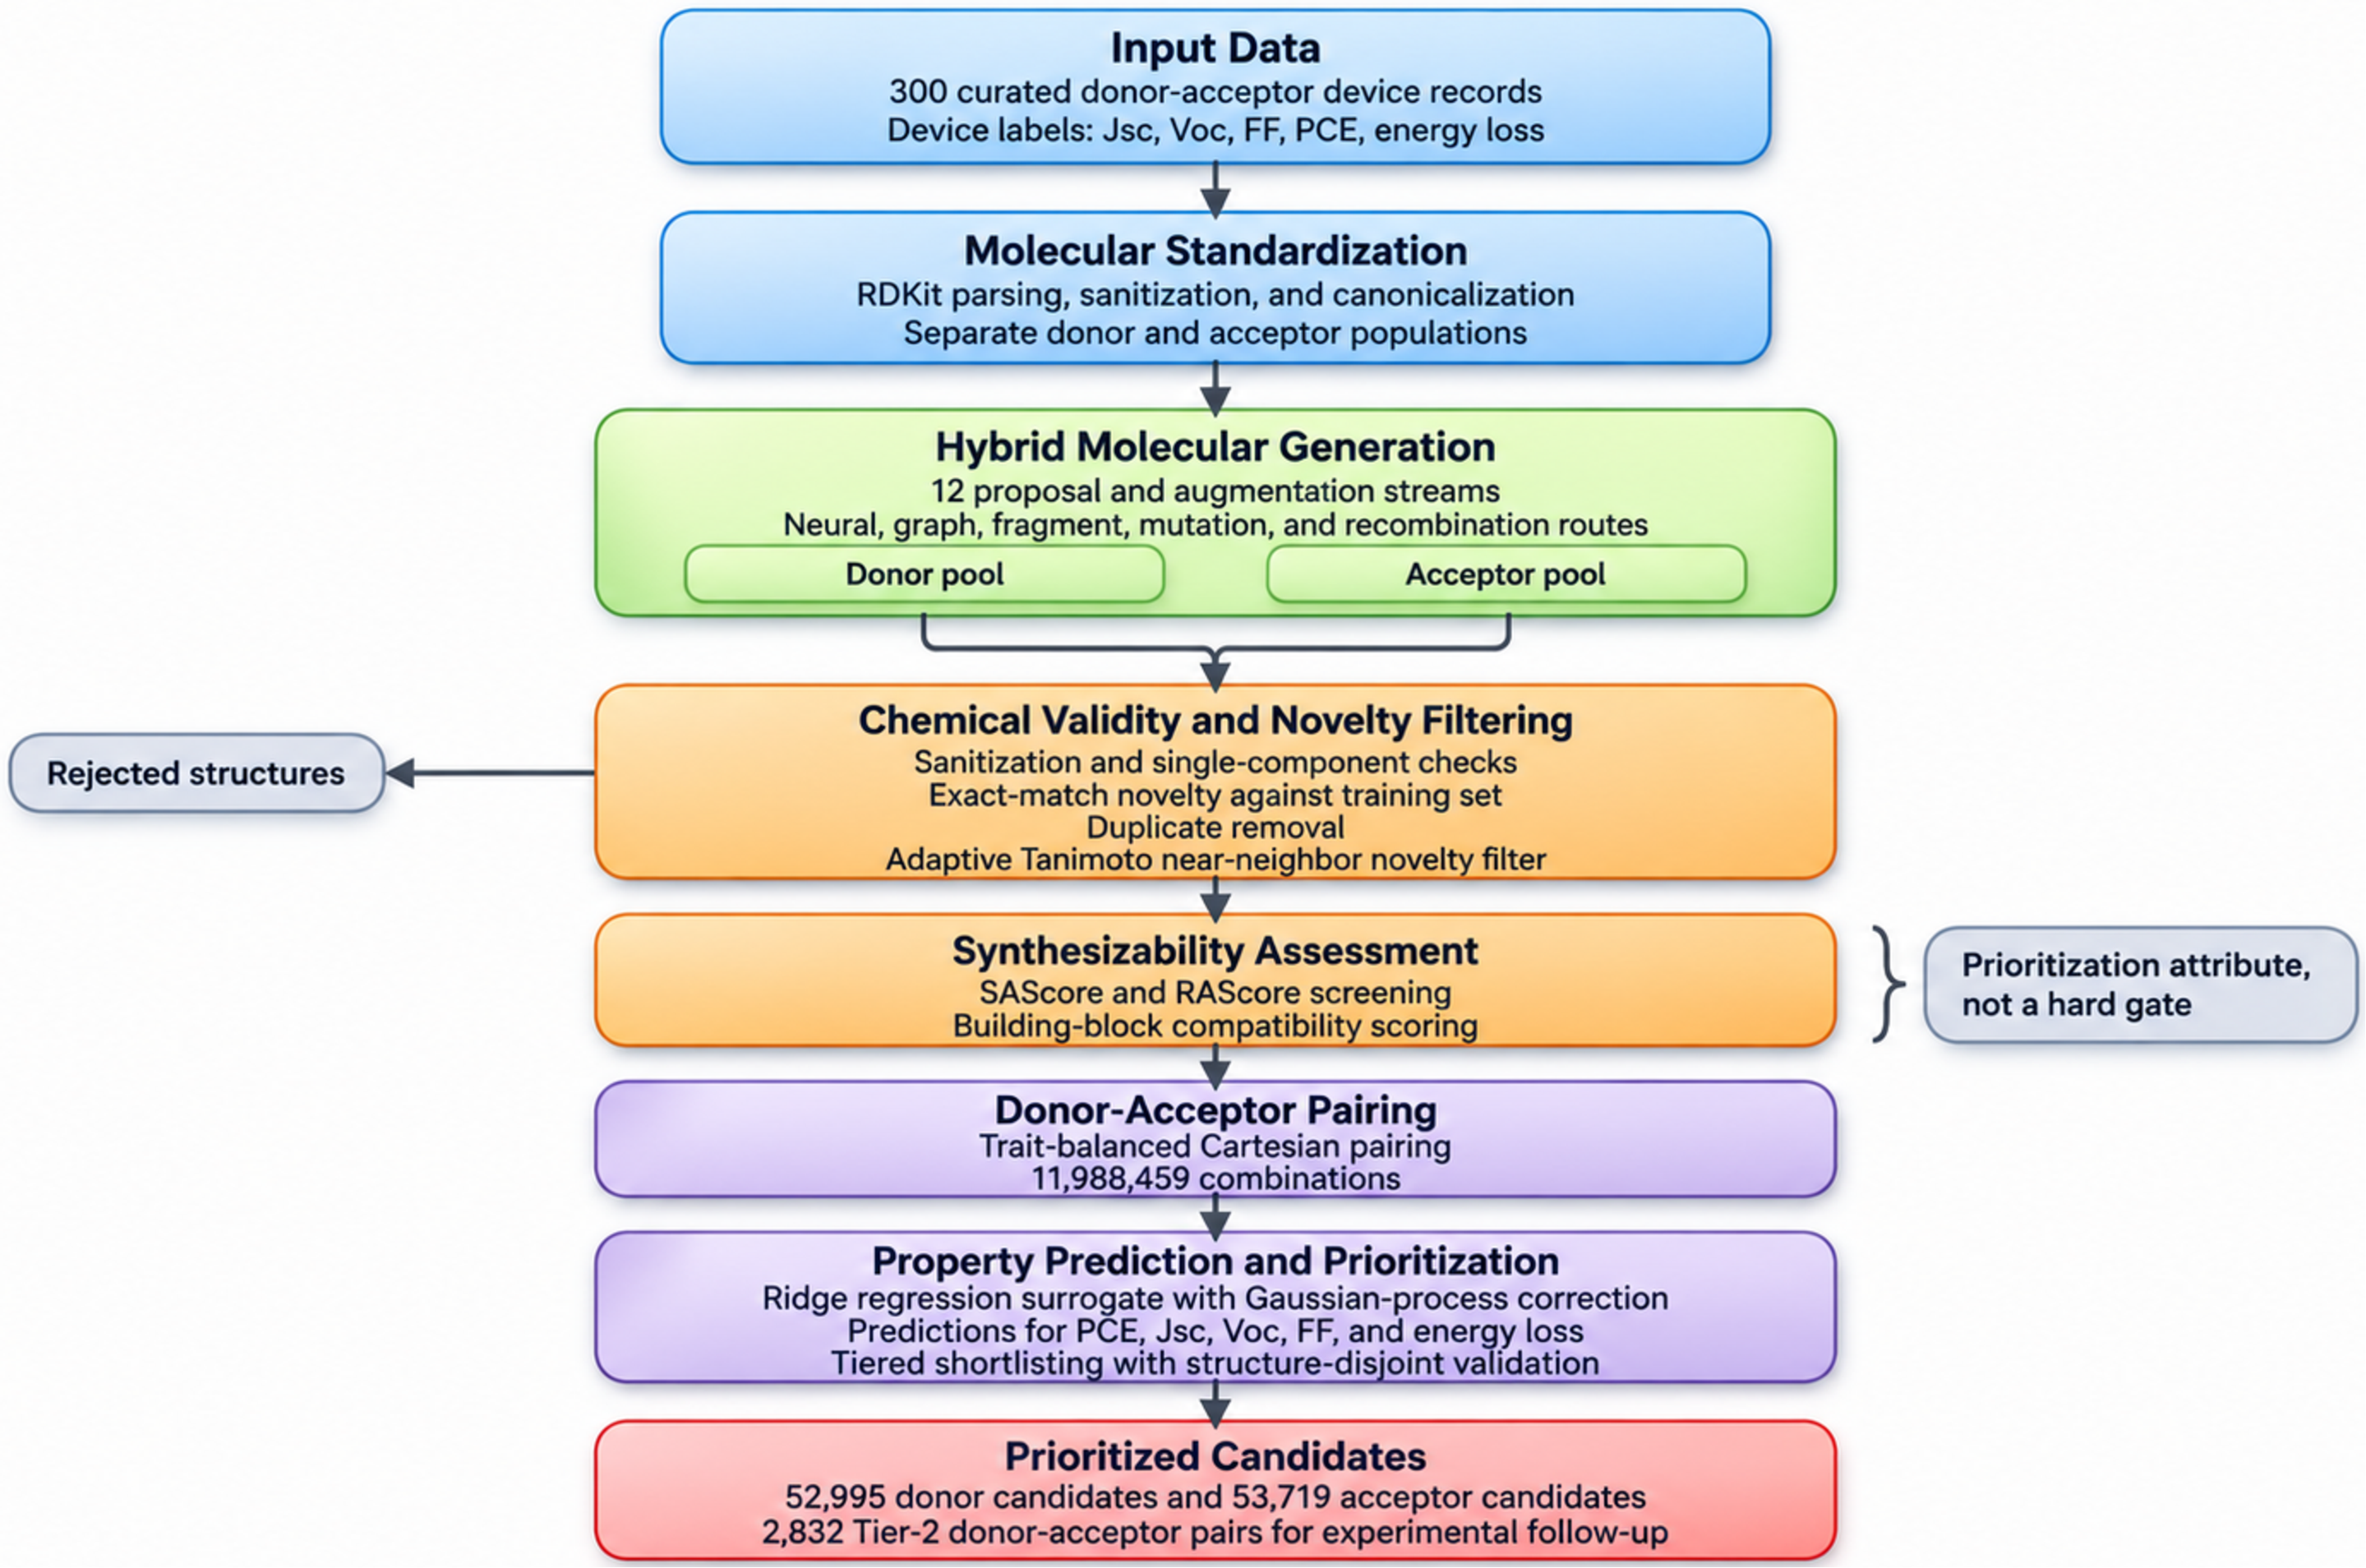
\includegraphics[width=10cm]{figures/Scheme.pdf}
\caption{Schematic workflow of the computational donor–acceptor discovery pipeline. The multi-stage framework flows from input-device record standardization and hybrid molecular generation through chemical validity filtering, synthesizability assessment, and Cartesian donor–acceptor pairing, and concludes with surrogate machine-learning property prediction and candidate shortlisting for experimental validation.}
\label{fig:scheme}
\end{figure}

Broad property-specific plausibility intervals were applied as safeguards against extreme extrapolation: $[0,21]\%$ for \pce, $[0,30]$ mA cm$^{-2}$ for \jsc, $[0.25,0.85]$ for FF, and $[0.3,2.0]$ V for \voc. These intervals were inspected to ensure that boundary values did not dominate the predicted distributions. Device energy loss was treated separately as an additional physical quality-control prediction rather than as a replacement for the four principal device targets. Physically implausible training energy-loss values were excluded from the corresponding model-development subset. For candidate pairs, an energy-loss estimate below $0.25$ eV was recorded as unavailable rather than silently clipped upward, consistent with the physical lower bound for OPV energy loss \cite{benduhn}. This policy preserves a transparent distinction between a value that satisfies the defined physical screen and one that lies outside the supported prediction domain.

The final prioritization retained the continuously predicted \jsc, \voc, FF, \pce, and energy-loss values, along with molecular novelty and synthetic-practicality indicators. Pair-level compatibility was obtained by combining the donor- and acceptor-level building-block compatibility scores. Candidates were thus ranked as a multi-criterion set for follow-up rather than declared experimentally high-performing solely based on a single predicted response. In particular, a predicted \pce\ is a screening quantity derived from a model trained on curated paired-device records and must not be interpreted as a measured efficiency for an untested donor--acceptor pair. The multi-stage sequential workflow, integrating molecular standardization, chemical novelty filtering, synthesizability scoring, and surrogate-based property predictions is shown in Figure \ref{fig:scheme}.

\section{Results and Discussion}

We developed a generative molecular design workflow to expand the accessible chemical space of donor and acceptor materials for OPVs while simultaneously considering structural novelty, synthetic accessibility, and device-relevant screening criteria. The resulting libraries were assessed at both the molecular and donor--acceptor-pair levels. Throughout this section, predicted device properties are interpreted as prioritization tools rather than as replacements for device fabrication and measurement. This distinction is particularly important for OPVs, where morphology, interfacial energetics, and processing conditions strongly influence device performance.

\subsection{Scale and Composition of the Generated Molecular Library}
A diverse ensemble of 12 generative approaches was employed to explore donor and acceptor chemical space, including character- and graph-based GANs, conditional and multi-objective variants, active- and reinforcement-learning strategies, transformer- and junction-tree-based generators, a variational autoencoder, a CoCoGraph-constrained model, and transfer learning and training-set augmentation approaches. The molecular candidates produced by these strategies were pooled prior to molecular standardization. Following canonicalization and removal of 
exact duplicates, the final library comprised $n_{\mathrm{donor}} = 52{,}995$ unique donor structures and $n_{\mathrm{acceptor}} = 53{,}719$ unique acceptor structures. The resulting libraries were fully valid, unique, and free of exact matches to the reference set. Because validity was enforced as part of the generation and filtering pipeline, these criteria primarily establish the integrity of the final molecular collection rather than serve as independent measures of generative performance.

Exact-match novelty alone, however, does not quantify the structural distance of the generated molecules from the reference chemical space. We therefore evaluated the nearest-neighbor Tanimoto similarity,
\begin{equation}
S_{\mathrm{NN}} = \max_{j \in \mathrm{train}} T(\mathrm{fp}_i,\mathrm{fp}_j),
\end{equation}
using radius-2, 2048-bit Morgan fingerprints. The mean $S_{\mathrm{NN}}$ across the complete generated libraries was $0.171$ for donors and $0.199$ for acceptors, while $97.0\%$ of donor structures and $99.9\%$ of acceptor structures had $S_{\mathrm{NN}} < 0.5$. Combined with the absence of exact matches to the reference set, these results indicate that the generated libraries extend beyond simple analogical reproduction and encompass substantially distinct regions of molecular chemical space. The extent of this structural separation should nevertheless be interpreted in the context of the chosen fingerprint representation and similarity threshold, as different fingerprint types or radius settings may yield different absolute similarity values for the same molecular pairs.

\subsection{Adversarial Training Dynamics and Convergence}
The adversarial models were monitored using the discriminator and generator losses together with discriminator classification accuracy. For the standard binary minimax GAN objective, an ideal balanced state corresponds to $\mathcal{L}_D = \mathcal{L}_G = \ln 2 \approx 0.693$ and a discriminator accuracy of approximately 50\%, indicating that generated and reference molecules cannot be reliably distinguished based on the learned representation.

\begin{figure}[!htb]
\centering
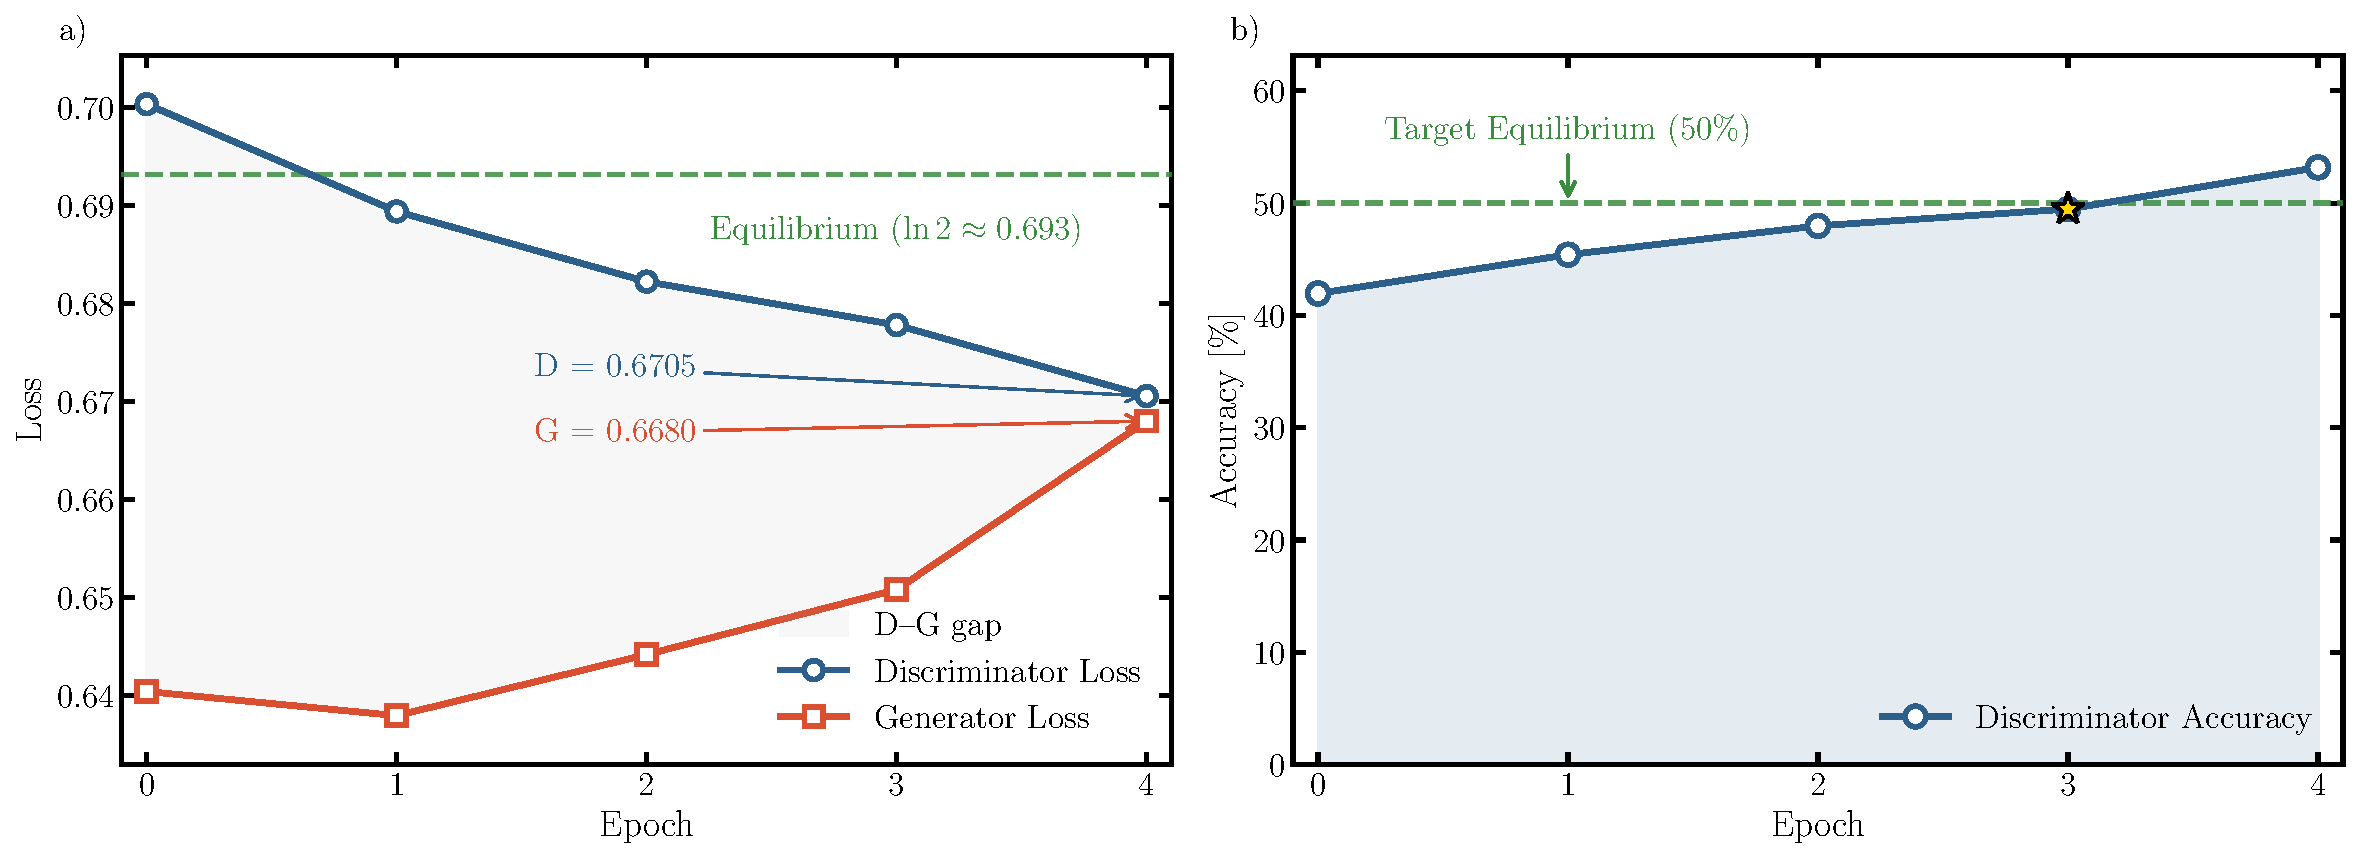
\includegraphics[width=16 cm]{figures/gan_training_donor_optimized.pdf}
\caption{(a) Evolution of discriminator loss ($\mathcal{L}_D$) and generator loss ($\mathcal{L}_G$) during donor-library generation; the dashed line denotes $\ln 2$, the characteristic loss of a balanced binary adversarial game. (b) Discriminator accuracy during donor-library generation; accuracy approaching 50\% indicates limited ability to distinguish generated structures from reference structures.}
\label{fig:G_loss_D_accuracy_donor}
\end{figure}

For the donor model, the discriminator loss decreased from 0.70 to 0.671 while the generator loss increased from 0.64 to 0.668 over five training epochs (Figure \ref{fig:G_loss_D_accuracy_donor}a). The corresponding acceptor model showed a similar evolution, with the discriminator loss converging to 0.676 and the generator loss to 0.649 (Figure 
\ref{fig:G_loss_D_accuracy_acceptor}a). Both models therefore approached the expected balanced-adversarial regime, with final losses lying within approximately $\pm 0.03$ of $\ln 2$. Discriminator accuracy evolved from 41.96\% to 53.18\% for donors (Figure \ref{fig:G_loss_D_accuracy_donor}b) and reached 51.91\% for acceptors (Figure \ref{fig:G_loss_D_accuracy_acceptor}b), remaining close to the 50\% equilibrium value in both cases.

\begin{figure}[!htb]
\centering
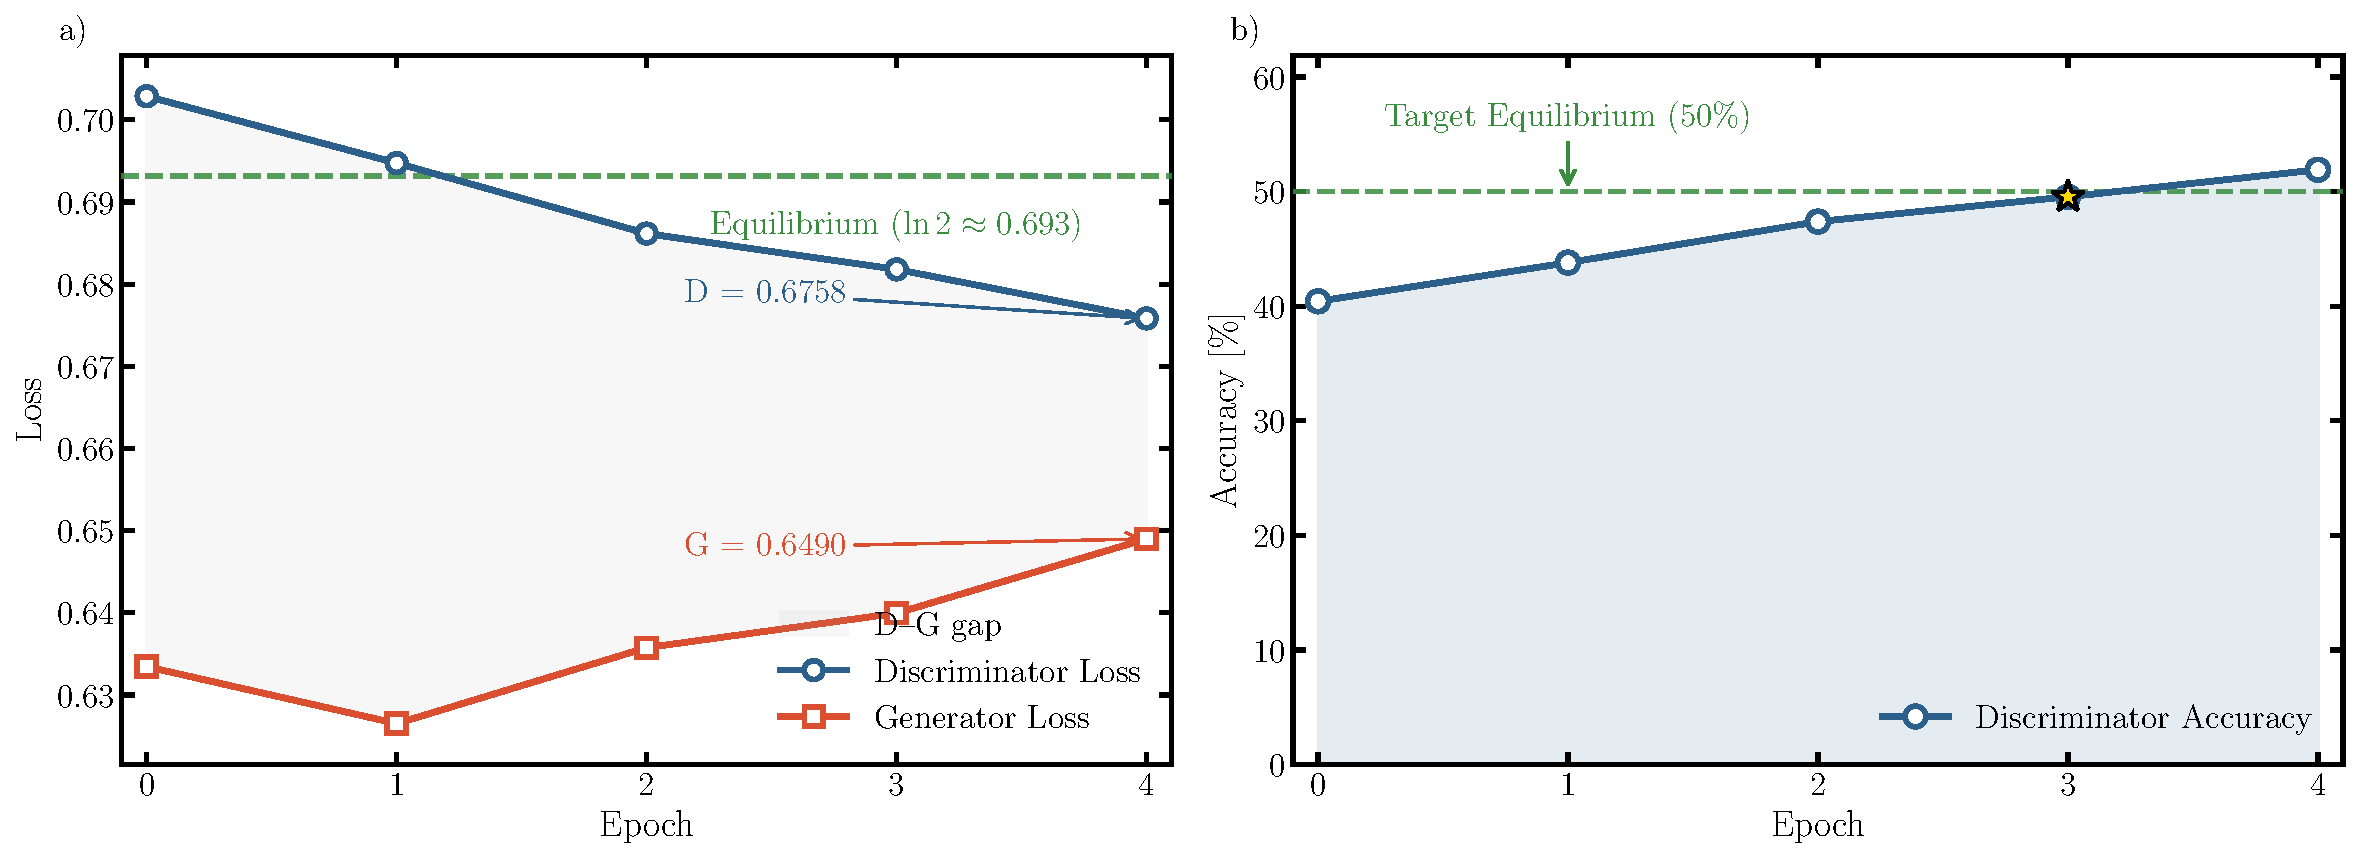
\includegraphics[width=16 cm]{figures/gan_training_acceptor_optimized.pdf}
\caption{(a) Evolution of discriminator loss ($\mathcal{L}_D$) and generator loss ($\mathcal{L}_G$) during acceptor-library generation; the dashed line denotes $\ln 2$. (b) Discriminator accuracy during acceptor-library generation.}
\label{fig:G_loss_D_accuracy_acceptor}
\end{figure}

Training was terminated after five epochs using an early-stopping criterion designed to prevent the discriminator from persistently dominating. Training was monitored for substantially sub-equilibrium discriminator losses ($\mathcal{L}_D < 0.45$), which were taken as an indication that the discriminator was becoming disproportionately strong relative to the generator. The final models therefore represent the training state selected by the adversarial convergence criterion rather than by an arbitrary fixed-epoch cutoff. Overall, the loss and accuracy trajectories are consistent with stable adversarial training, with no evidence of severe discriminator domination or generator collapse.

\subsection{Chemical-Space Coverage, Novelty, and Structural Diversity}
The structural and physicochemical characteristics of the generated libraries were evaluated using a representative sample of $n = 20{,}000$ molecules from each molecular class. Chemical-space coverage was assessed using nearest-neighbor similarity to the reference set, descriptor-based property agreement, and internal structural diversity, providing complementary measures of how closely the generated molecules resemble the training chemical space while retaining structural variation.

Internal diversity was quantified for each sampled molecule as
\begin{equation}
\mathrm{IntDiv}_i = 1 - \max_{j \neq i,\; j \in \mathcal{G}} 
T(\mathrm{fp}_i, \mathrm{fp}_j),
\end{equation}
where $T(\mathrm{fp}_i, \mathrm{fp}_j)$ denotes the Morgan--Tanimoto similarity between radius-2, 2048-bit molecular fingerprints and $\mathcal{G}$ denotes the complete generated library for the corresponding molecular class. Thus, $\mathrm{IntDiv}_i$ is the structural distance between molecule $i$ and its most similar distinct generated neighbor. Unlike the average-pairwise internal-diversity definition used in the MOSES benchmark \cite{moses}, this nearest-neighbor formulation provides a molecule-level diversity value that can 
be represented directly in the chemical-space analysis without involving a classifier or probabilistic scoring function. Each sampled molecule was compared against the complete donor ($52{,}995$ molecules) or acceptor ($53{,}719$ molecules) generated library. The resulting mean $\mathrm{IntDiv}_i$ values were $0.485$ for donors and $0.491$ for acceptors, indicating substantial structural heterogeneity in both libraries. This conclusion is further supported by Bemis--Murcko scaffold diversity values of $0.768$ and $0.824$ for donors and acceptors, respectively, demonstrating that the generated molecules span multiple distinct scaffold families rather than being concentrated around a limited set of core structures. These complementary molecular-level characteristics are jointly visualized in Figure~\ref{fig:combined_space_analysis}.

\begin{figure}[!htb]
\centering
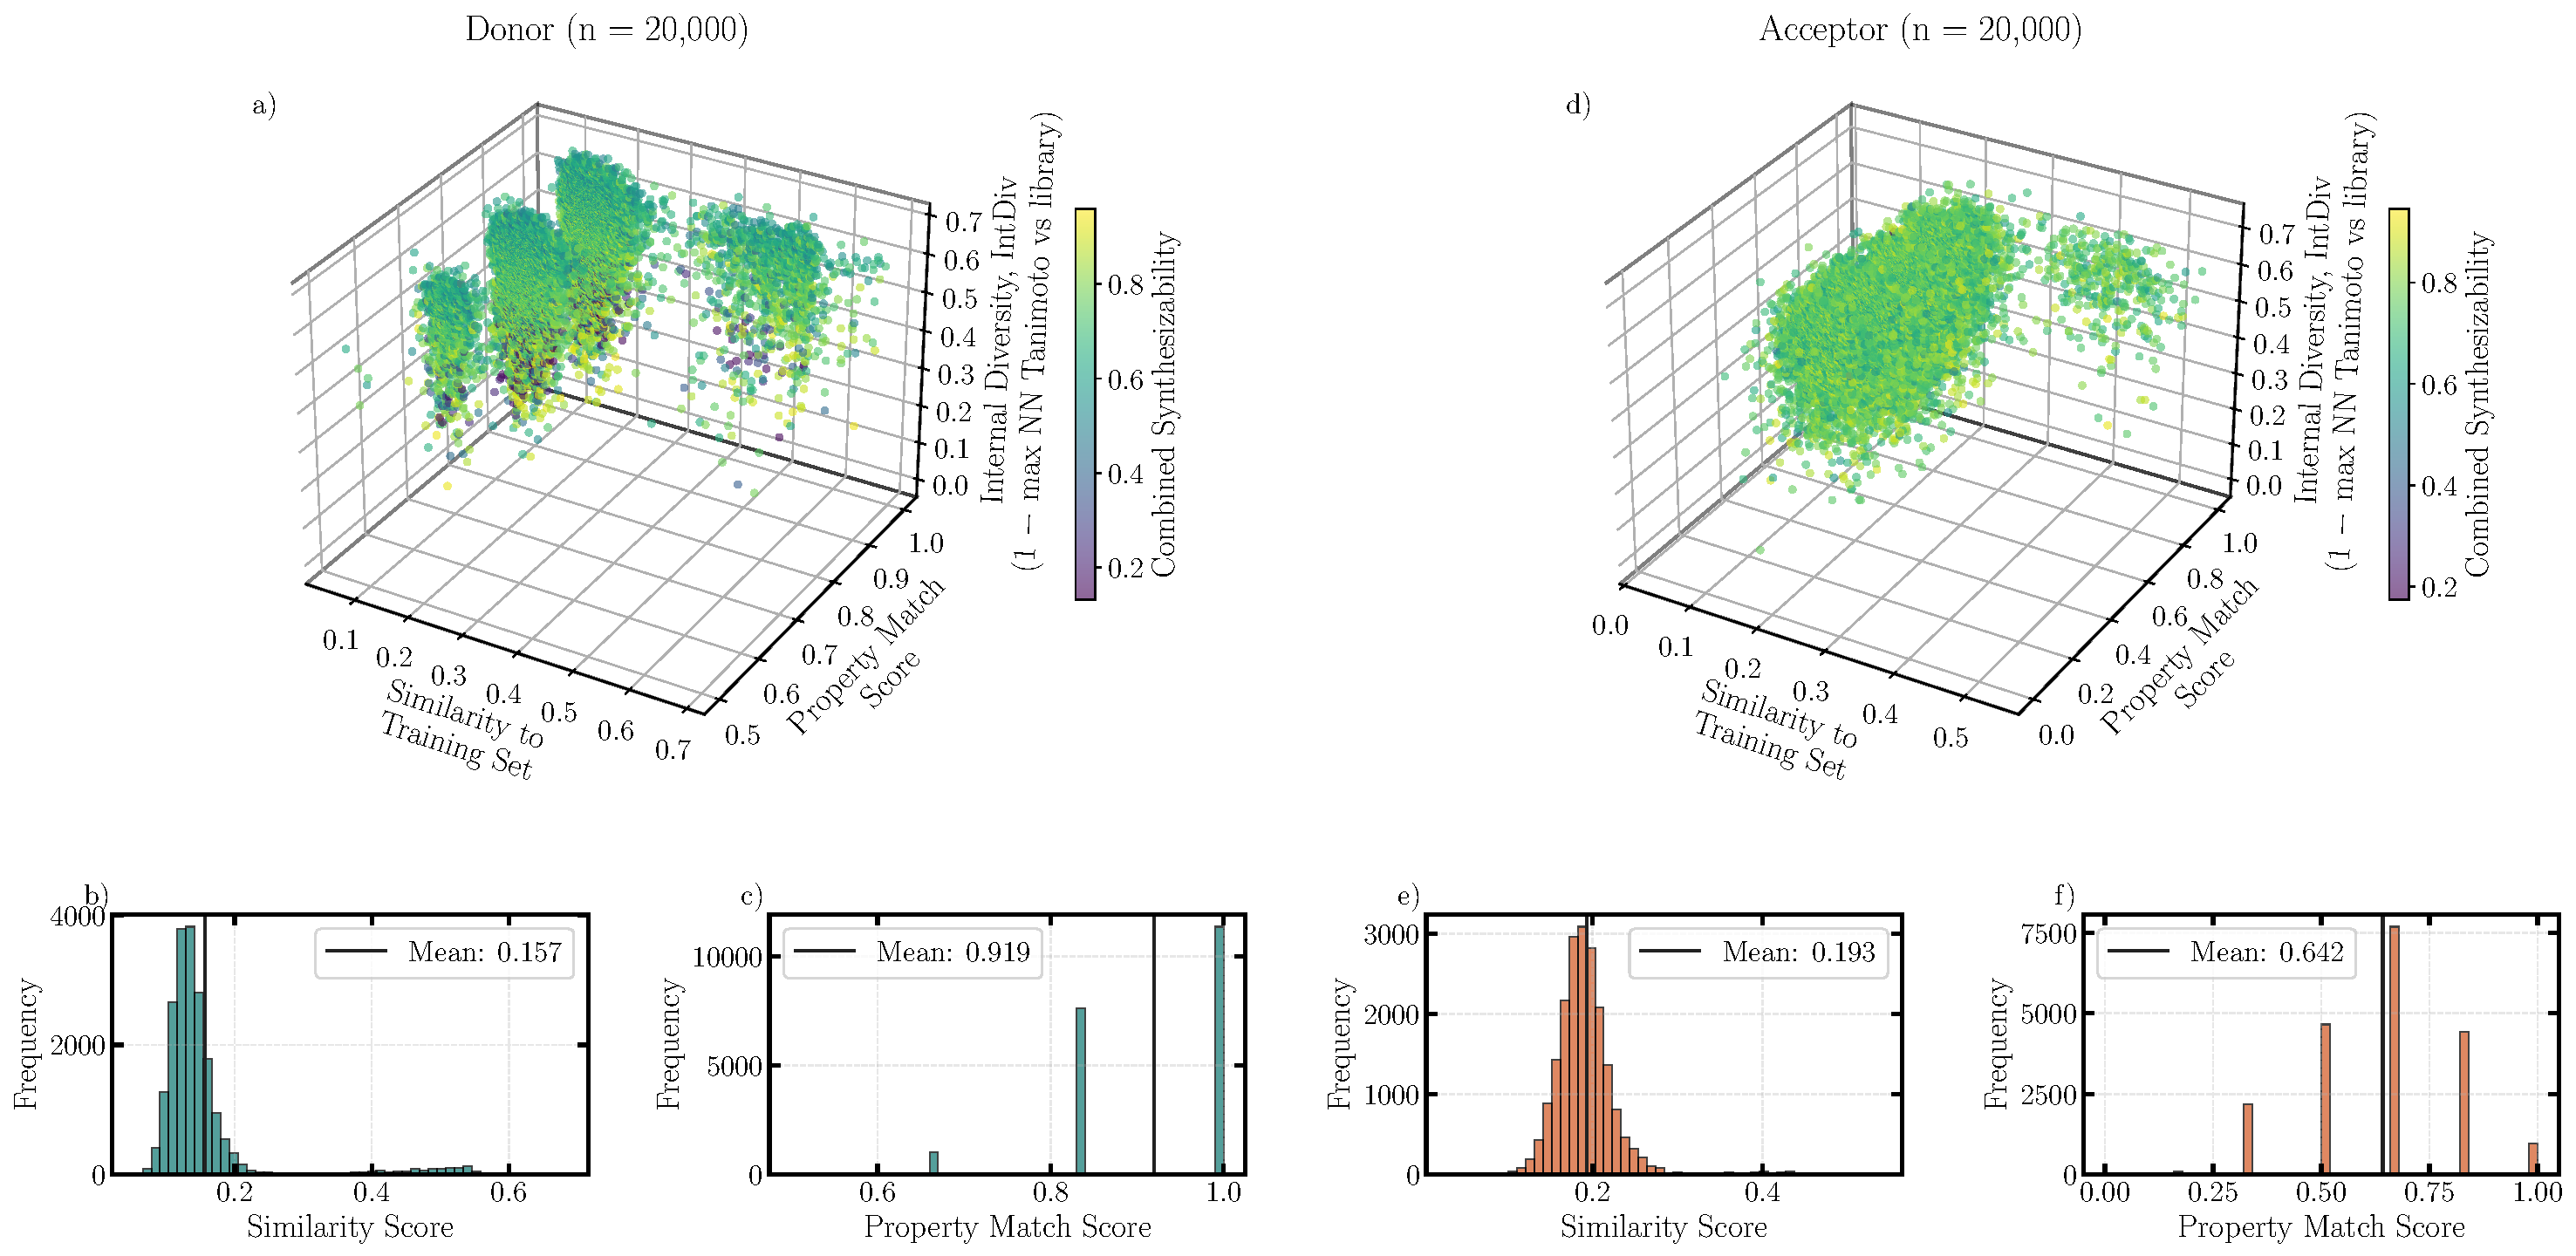
\includegraphics[width=16 cm]{figures/combined_space_analysis.pdf}
\caption{Combined four-dimensional chemical-space analysis of generated (a) donor and (b) acceptor candidates. A reproducible subset of $20{,}000$ structures from each complete library is displayed. The $x$-, $y$-, and $z$-coordinates represent nearest-neighbor similarity to the training set, descriptor-based property-match score, and pointwise internal diversity relative to the complete generated library, respectively. Point color represents the combined synthesizability score.}
\label{fig:combined_space_analysis}
\end{figure}

The relationship between the generated and reference chemical spaces was further examined using several distribution-level distance measures. Because these metrics are defined in different embedding spaces, their absolute values should not be compared directly across metrics. A fingerprint-based Fr\'{e}chet distance obtained from a low-dimensional projection of Morgan fingerprints was $25.2$ for donors and $17.0$ for acceptors. A property-embedding Fr\'{e}chet distance (PFD), calculated in the latent representation of an OPV-relevant property-prediction model, was $444.3$ for donors and $428.0$ for acceptors. The PFD provides the most chemically relevant measure of distributional similarity in the present context because its representation is learned from OPV-related molecular properties. To calibrate the fingerprint-space distance, we evaluated the same metric over 200 random 50/50 train--train splits of each reference library. The resulting split-half values were low (means: $0.24$ for donors and $0.12$ for acceptors; Figure~S1), whereas the train-vs-generated distances exceeded this sampling baseline by approximately $107\times$ and $140\times$, respectively. The observed separation therefore reflects a reproducible distributional shift rather than finite-sample variation. An analogous baseline was not available for PFD because the embedding-model checkpoint was not retained; PFD is consequently interpreted comparatively rather than against an absolute threshold.

For comparison with broader generative-chemistry benchmarks, the Fr\'{e}chet ChemNet Distance (FCD) was also evaluated using the published ChemNet embedding \cite{fcd}. The resulting donor value was $26.5$. FCD was not available for the acceptor library because the ChemNet molecular encoder imposes a maximum SMILES length of 350 characters, which was exceeded by the acceptor structures considered here. This limitation reflects the range of applicability of the external ChemNet representation and does not indicate a deficiency in the generated acceptor structures.

Agreement with the reference chemical space was additionally assessed using six conventional molecular descriptors: molecular weight, $\log P$, topological polar surface area (TPSA), hydrogen-bond acceptor and donor counts, and rotatable-bond count. A descriptor-based property-match fraction yielded mean values of $0.919$ for donors and $0.642$ for acceptors. Because this score is based on discrete descriptor criteria, it was complemented by continuous distributional measures. The normalized 1-Wasserstein distance was $\overline{W}_1 = 1.564$ for donors and $2.192$ for acceptors, while the corresponding mean Mahalanobis distances from the reference descriptor manifold were $\overline{D}_M = 448$ and $1787$, respectively.

Taken together, these complementary analyses indicate that both generated libraries possess substantial internal structural diversity while remaining chemically related to the reference domain. The acceptor library exhibits greater separation from the reference descriptor distribution than the donor library, particularly in the Mahalanobis and Wasserstein measures. This is consistent with the broader structural diversity of NFA chemotypes relative to the donor structures represented in the curated training set. Consequently, property predictions for acceptor candidates should be regarded as more extrapolative than those for donor candidates, an effect assessed quantitatively via structure-disjoint validation of the screening surrogate in Section~\ref{sec:validation}.

\subsection{Synthetic Accessibility and TANGO-Inspired Screening}
The synthetic feasibility of the generated molecular libraries was evaluated using complementary structure-based and retrosynthesis-informed criteria. The Ertl--Schuffenhauer synthetic-accessibility score (\texttt{SAScore}), ranging from 1 (more accessible) to 10 (more difficult) \cite{sascore}, was combined with the \texttt{RAscore} retrosynthesis-feasibility classifier, for which larger values indicate greater predicted accessibility \cite{rascore}. Molecules satisfying \texttt{SAScore} $\leq$ 6.0 and \texttt{RAscore} $\geq$ 0.5 were retained as synthetically promising candidates.

Across all generated libraries, the mean \texttt{SAScore} was 3.91 for donors and 3.64 for acceptors, indicating generally favorable synthetic accessibility in both libraries. The corresponding mean \texttt{RAScore} values were 0.674 and 0.776, respectively. On applying the operational two-criterion screen of \texttt{SAScore} $\leq$ 6.0 and \texttt{RAScore} $\geq$ 0.5, 85.0\% of donor structures ($45{,}066/52{,}995$) and 99.3\% of acceptor structures ($53{,}351/53{,}719$) passed the screen. These results suggest that a large fraction of the generated structures occupy regions of chemical space compatible with commonly encountered synthetic complexity and retrosynthetic feasibility measures (Figure~\ref{fig:sascore_rascore_tango_4d_donor}a,b).

\begin{figure}[!htb]
\centering
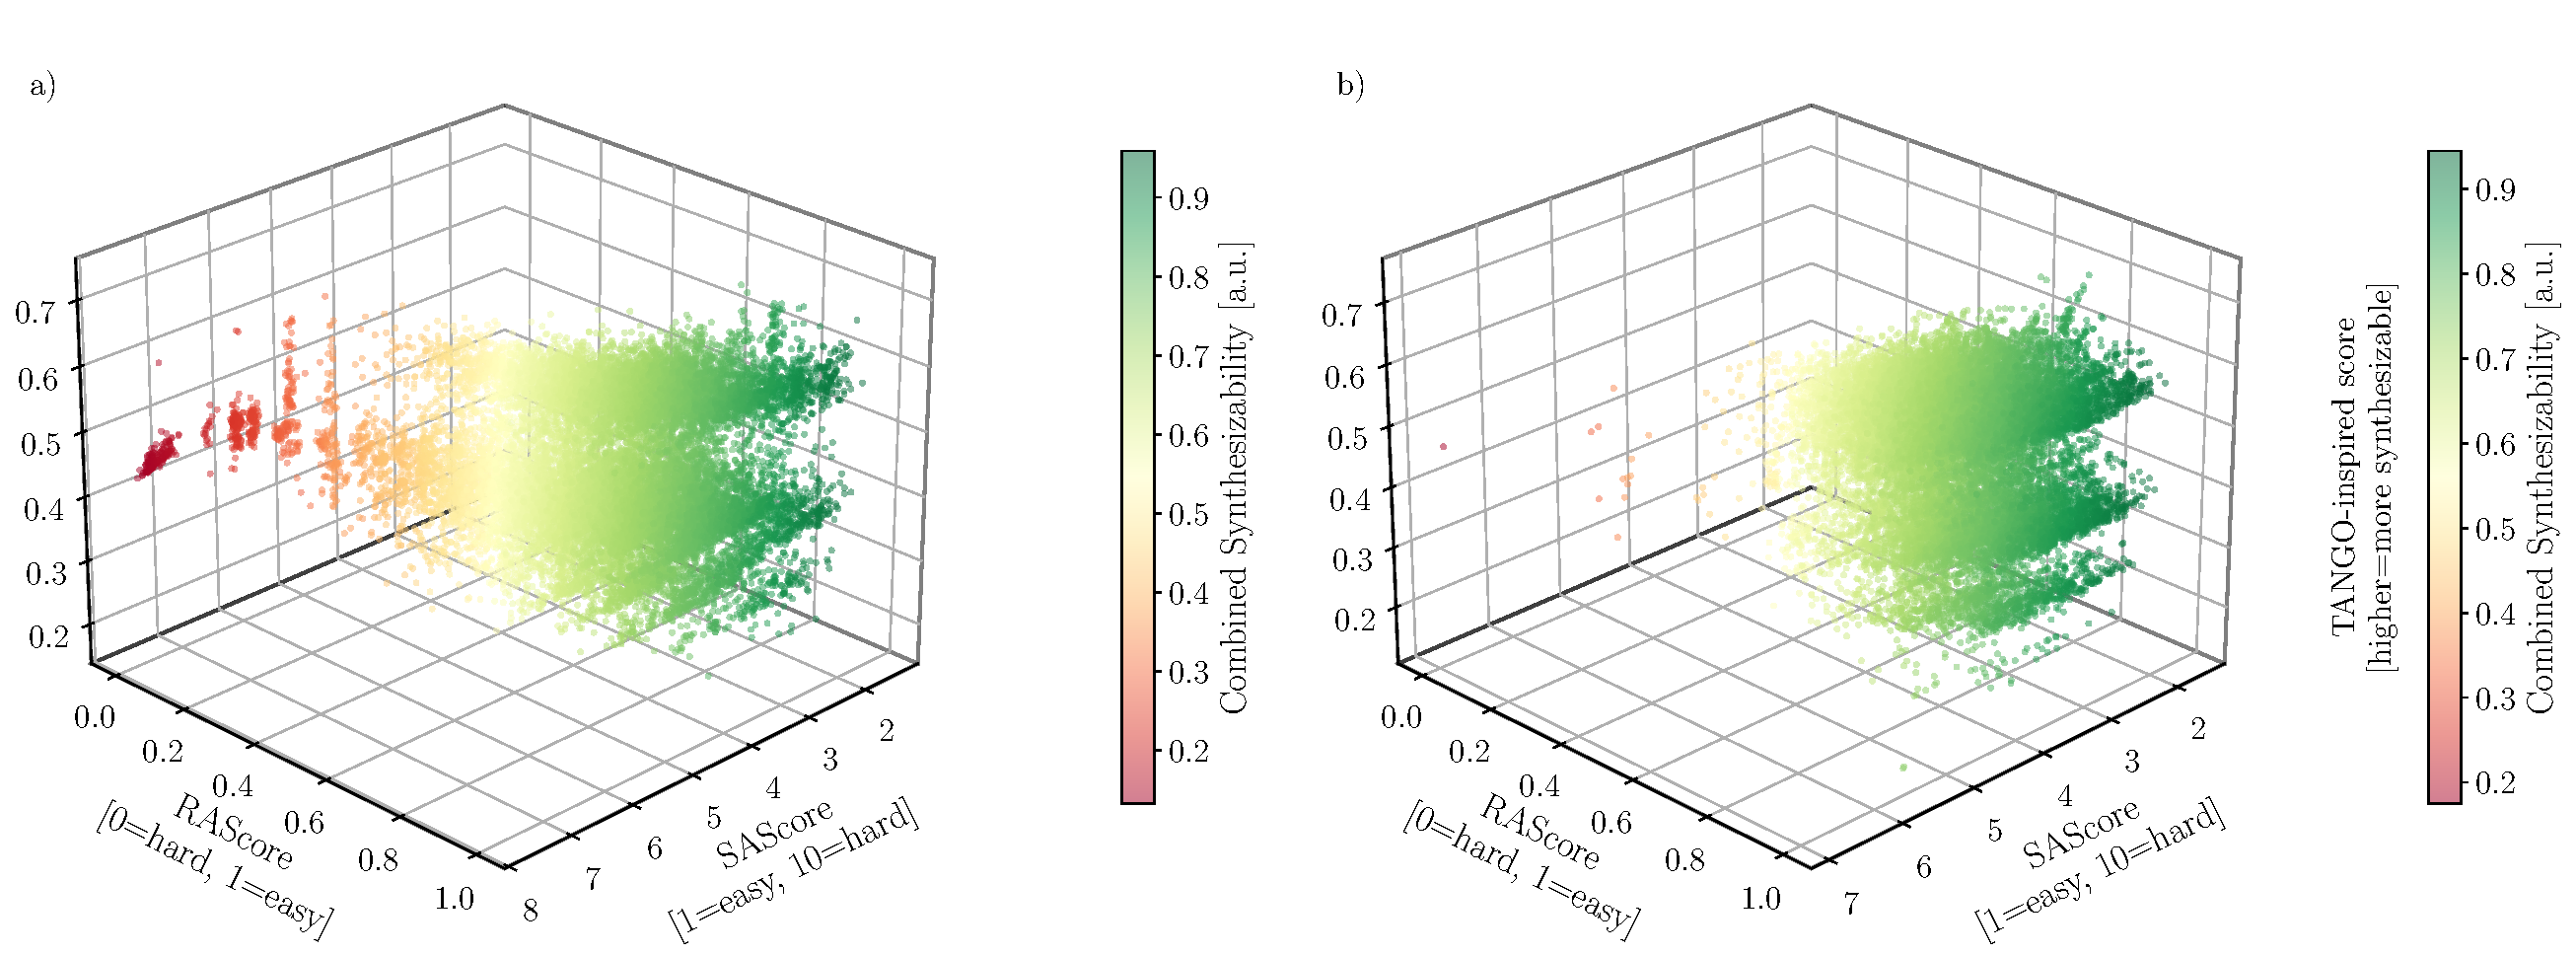
\includegraphics[width=16 cm]{figures/sascore_rascore_tango_4d_combined.pdf}
\caption{Joint view of synthetic accessibility, retrosynthetic feasibility, and building-block compatibility for generated (a) donor and (b) acceptor candidates. Point color encodes the continuous combined-synthesizability score. The inset in each panel reports the separate three-criterion visual summary for structures satisfying \texttt{SAScore} $\leq$ 6.0, \texttt{RAScore} $\geq$ 0.5, and TANGO-inspired score $\geq$ 0.5; the operational accessibility screen reported in the text uses \texttt{SAScore} and \texttt{RAScore} only.}
\label{fig:sascore_rascore_tango_4d_donor}
\end{figure}

The interpretation of \texttt{RAscore} requires particular caution in the present application. The model was developed from retrosynthetic information associated with \texttt{ChEMBL}-like chemical space, \cite{rascore} \adref\ whereas many OPV donor and acceptor architectures contain extended conjugated frameworks and structural motifs that are underrepresented in that domain. Accordingly, \texttt{RAscore} values are used here as comparative screening indicators rather than as calibrated probabilities that a valid synthetic route exists \cite{rascore}.

A complementary building-block-overlap heuristic was used to assess the relationship between generated structures and a curated OPV building-block space. The score was defined as
\begin{equation}
S = \alpha \cdot \mathrm{FMS} + (1-\alpha) \cdot \mathrm{BB\text{-}Tanimoto},
\end{equation}
with $\alpha = 0.5$, where $\mathrm{FMS}$ denotes a fragment-match component and $\mathrm{BB\text{-}Tanimoto}$ quantifies structural overlap with the reference building-block collection. The resulting mean scores were 0.463 for donors and 0.502 for acceptors. This quantity is explicitly treated as a TANGO-inspired heuristic rather than as the published TANGO reward \cite{tango}. In particular, it does not incorporate the retrosynthetic search and starting-material constraints underlying the original TANGO framework and therefore should not be interpreted as a probability of successful synthesis.

Finally, a focused retrosynthetic audit was performed for a shortlist of 864 molecules. Using \texttt{RAscore} as the available retrosynthetic screening backend, 661 candidates (76.5\%) were classified as route-findable. This result provides further evidence that a substantial fraction of the shortlisted structures have plausible retrosynthetic accessibility according to the employed model. However, because the higher-fidelity \texttt{AiZynthFinder} Monte Carlo tree-search backend and its associated stock and policy assets were not available for this analysis, the result should be regarded as an indicative computational screen rather than confirmation of experimentally executable synthetic routes.

\subsection{Device-Property Prediction and Its Limitations}
Device-relevant properties, including power-conversion efficiency (PCE), short-circuit current density (\jsc), fill factor (FF), and open-circuit voltage (\voc), were estimated using a descriptor-based screening surrogate trained on the 300-entry curated reference set containing experimental and DFT-derived OPV data. \cite{das2024predictive} \adref\ The model combines ridge regression with isotonic recalibration and a Gaussian-process residual correction, and was developed to provide a consistent ranking of donor--acceptor combinations rather than to quantitatively predict experimentally realized device performance. Accordingly, the predicted values are used throughout this work primarily for candidate prioritization.

Across 11{,}988{,}459 generated donor--acceptor pairs, the mean predicted values were PCE = 5.87\%, \jsc\ = 11.28 mA cm$^{-2}$, FF = 0.534, and \voc\ = 0.854 V. The corresponding maximum predicted values were 18.22\%, 27.70 mA cm$^{-2}$, 0.785, and 1.295 V, respectively 
(Figure~\ref{fig:device_properties_distribution_method1}a--d). All predictions remained within the physically imposed ranges of [0, 21]\% for PCE, [0, 30] mA cm$^{-2}$ for \jsc, [0.25, 0.85] for FF, and [0.3, 2.0] V for \voc, without accumulation at the boundaries. This indicates that the imposed bounds function primarily as safeguards against unphysical extrapolation rather than determining the overall shape of the predicted distributions.

\begin{figure}[!htb]
\centering
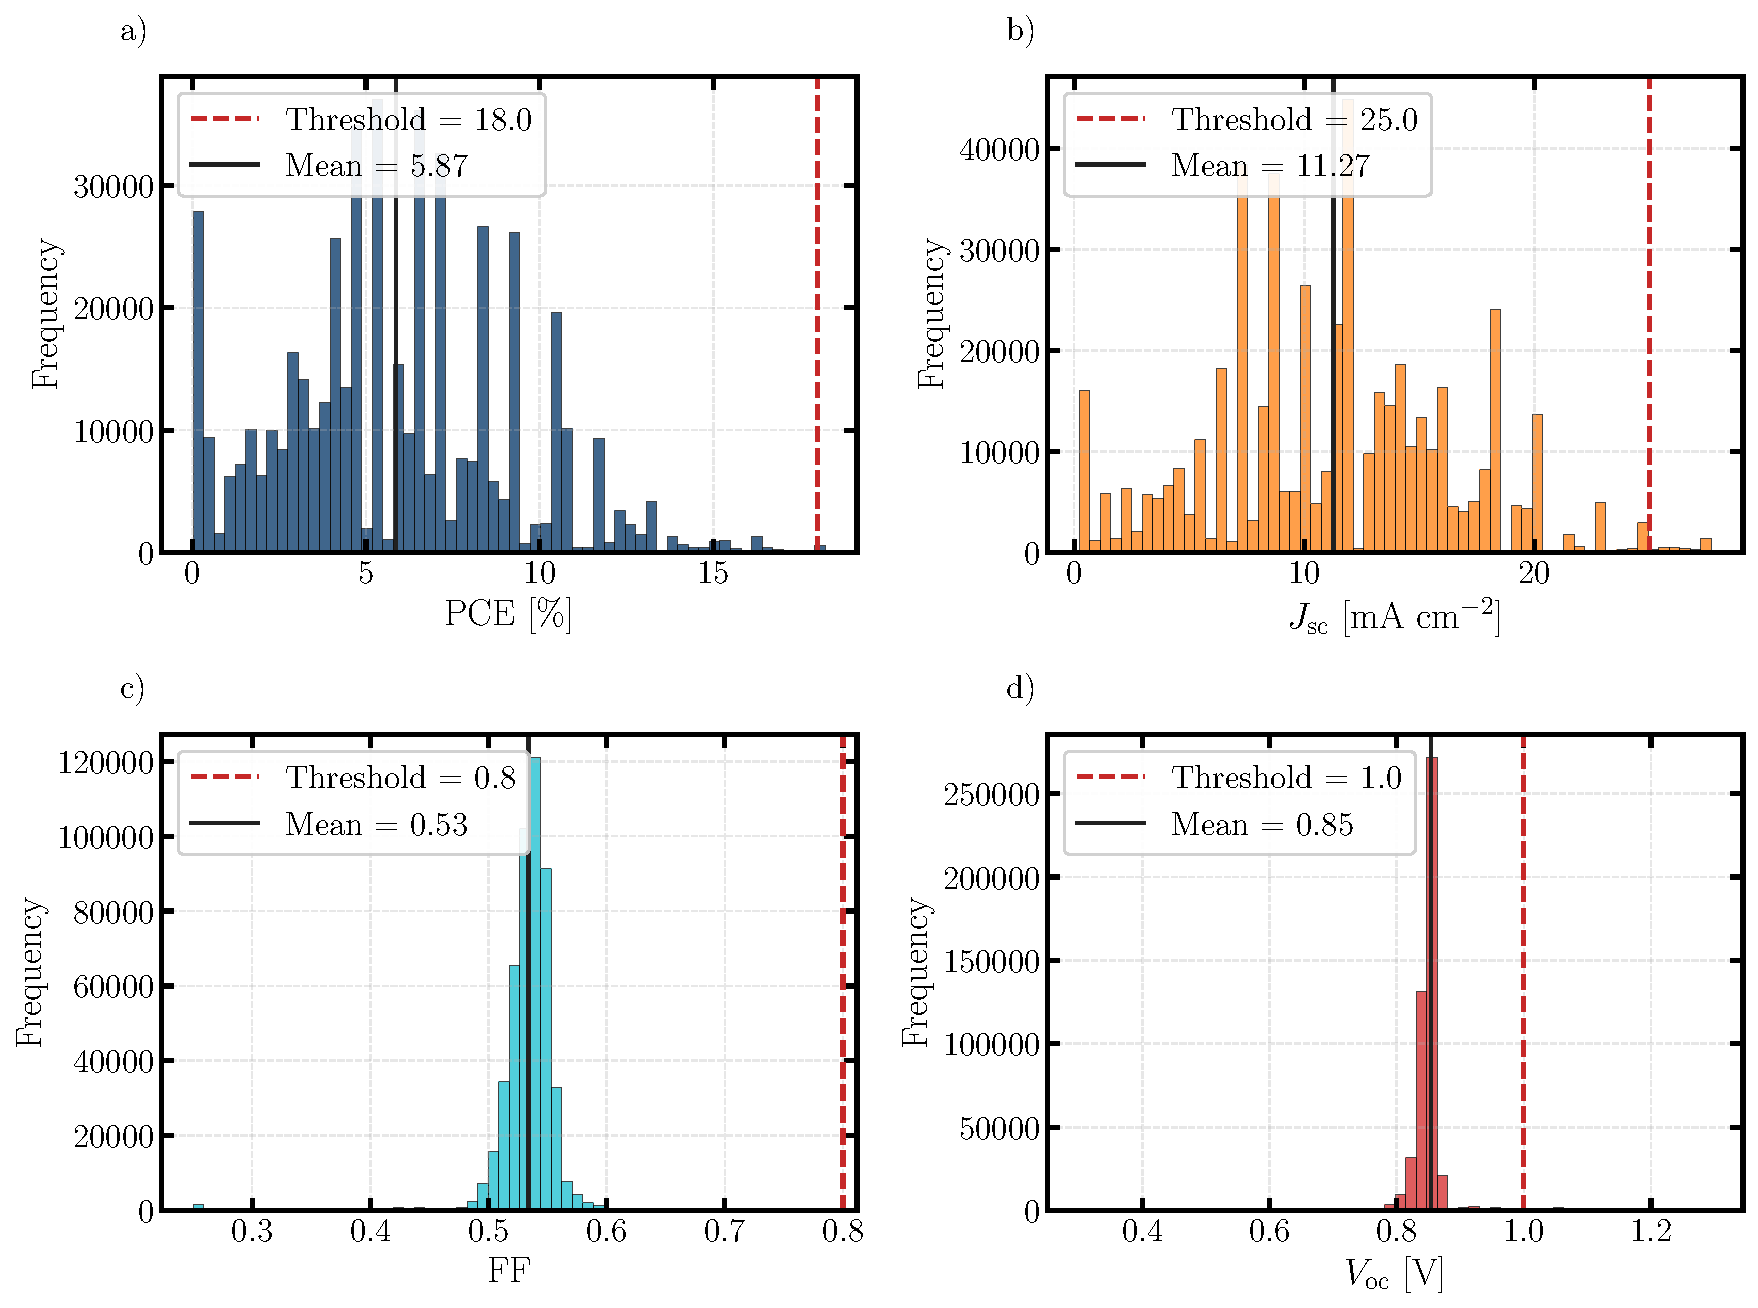
\includegraphics[width=16 cm]{figures/device_properties_distribution_method1_ridge_gp.pdf}
\caption{Predicted distributions of (a) PCE, (b) \jsc, (c) FF, and (d) \voc\ for generated donor--acceptor pairs. Values are used for relative candidate prioritization and should not be interpreted as experimentally verified device efficiencies.}
\label{fig:device_properties_distribution_method1}
\end{figure}

For context, experimentally demonstrated single-junction OPVs have surpassed 20\% efficiency \cite{recorddevice}, placing the predicted upper tail within the range of technologically relevant performance. Nevertheless, the substantially lower mean predicted values and the limited size and structural diversity of the labeled reference set emphasize that these predictions should not be interpreted as evidence of experimentally attainable efficiencies. Rather, they identify regions of the generated chemical space that warrant closer experimental or higher-fidelity computational evaluation.

\subsubsection{Structure-Disjoint Validation of the Screening Surrogate}\label{sec:validation}

The reliability of the surrogate was assessed using group-disjoint cross-validation in which structurally related molecules were excluded from the training data when evaluating the corresponding test set. Donor-disjoint, acceptor-disjoint, and Bemis--Murcko scaffold-disjoint splits were considered to provide a stringent assessment of transfer to previously unseen chemical structures.

The resulting performance was strongly target-dependent. For acceptor-side frontier-orbital properties (HOMO, LUMO, and $E_\text{g}$), held-out $R^2$ values ranged from 0.44 to 0.69, indicating meaningful generalization within the represented chemical space. In contrast, donor-side frontier-orbital predictions gave held-out $R^2$ values between $-0.33$ and $-0.25$ (Figure~\ref{fig:method1_disjoint_cv_r2}), reflecting the limited number of unique donor structures in the reference set and the resulting inability of the model to learn a robust donor structure--property relationship.

\begin{figure}[!htb]
\centering
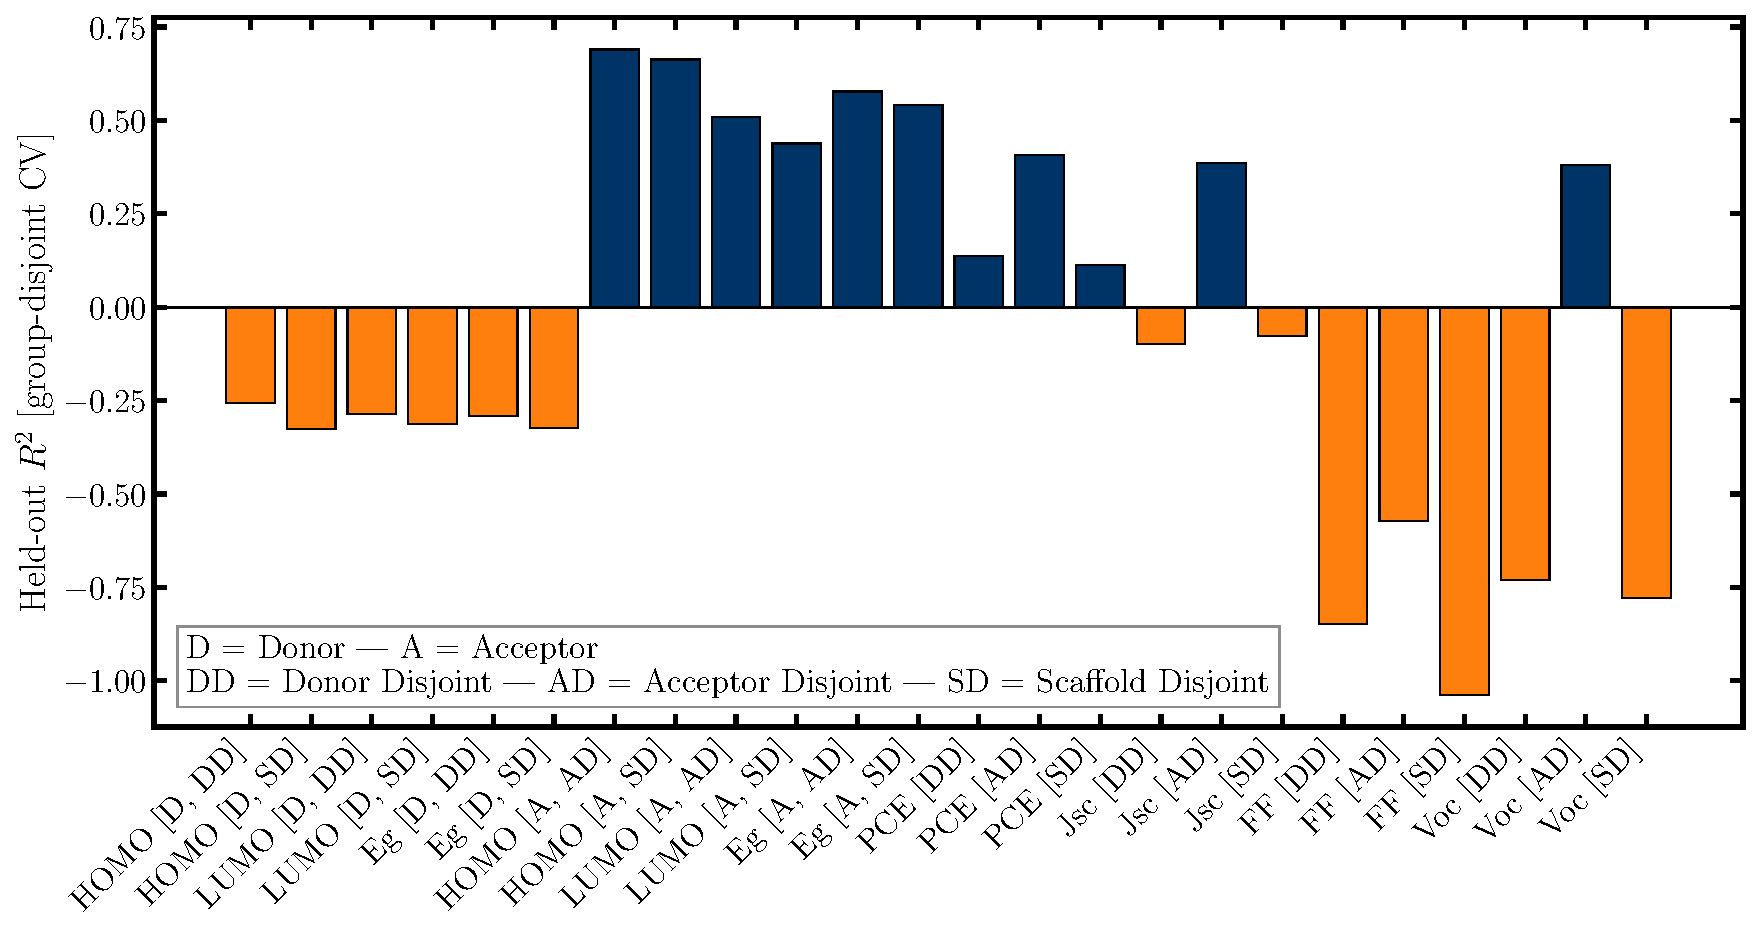
\includegraphics[width=16 cm]{figures/method1_disjoint_cv_r2.pdf}
\caption{Structure-disjoint validation of molecular and device-property 
predictions. Negative $R^2$ values indicate performance below that obtained by predicting the reference-set mean, identifying properties for which the present dataset does not support reliable extrapolation.}
\label{fig:method1_disjoint_cv_r2}
\end{figure}

Pair-level predictions showed intermediate performance. For PCE, held-out $R^2$ values ranged from 0.11 to 0.41, indicating a weak but measurable relationship under structure-disjoint evaluation. Predictions of \jsc\ were similarly limited, with performance becoming slightly negative under scaffold-disjoint testing. FF yielded negative held-out $R^2$ values across all three validation schemes (donor-disjoint: $-0.85$; acceptor-disjoint: $-0.57$; scaffold-disjoint: $-1.04$), indicating that the present model does not demonstrate reliable quantitative predictive accuracy for FF under structure-disjoint evaluation. \voc\ similarly performed poorly under donor-disjoint ($-0.73$) and scaffold-disjoint ($-0.78$) evaluation but achieved a positive held-out $R^2$ of 0.38 under acceptor-disjoint evaluation (Figure~\ref{fig:method1_disjoint_cv_r2}), indicating that its transferability is protocol dependent rather than uniformly negative. 

These validation results motivate using the surrogate primarily as a ranking and prioritization tool rather than as a predictive model of absolute device performance. Accordingly, the tiering criteria introduced below are interpreted as an exploratory composite prioritization heuristic rather than as validated predictive filters for structurally novel pairs. As a sensitivity analysis, removing the FF and \voc\ thresholds from Tier~2 increased the shortlist from 2{,}832 to 133{,}943 pairs (approximately 47-fold) and yielded 1{,}584 nominal Tier-1 pairs. Thus, FF and \voc\ provide substantial practical selectivity, but their predicted values should not be interpreted as reliable quantitative estimates for previously unseen chemistry.

\subsection{Pair-Level Screening and Tiered Shortlisting}
The generated donor--acceptor combinations were subsequently prioritized using the surrogate predictions together with a pair-compatibility score, $T_{\mathrm{pair}}$, derived from the donor- and acceptor-level building-block compatibility measures. Two nested screening criteria were applied:
\begin{equation}
\begin{aligned}
\mathrm{Tier\ 1}: \quad &
\mathrm{PCE} \geq 18\%, \quad
J_\mathrm{sc} \geq 25\ \text{mA\,cm}^{-2}, \quad
\mathrm{FF} \geq 0.75, \quad
V_\mathrm{oc} \geq 1.0\ \text{V}, \quad
T_{\mathrm{pair}} \geq 0.5,\\
\mathrm{Tier\ 2}: \quad &
\mathrm{PCE} \geq 14\%, \quad
J_\mathrm{sc} \geq 18\ \text{mA\,cm}^{-2}, \quad
\mathrm{FF} \geq 0.60, \quad
V_\mathrm{oc} \geq 0.85\ \text{V}, \quad
T_{\mathrm{pair}} \geq 0.35.
\end{aligned}
\end{equation}
No pair satisfied all Tier-1 criteria, whereas 2{,}832 donor--acceptor 
combinations met the Tier-2 requirements. Within this exploratory Tier-2 set, the mean predicted properties were PCE = 15.85\% (range 14.0--18.2\%), \jsc\ = 23.5 mA cm$^{-2}$, FF = 0.737, \voc\ = 0.864 V, and 
$T_{\mathrm{pair}}$ = 0.454. These pairs define a deliberately restrictive set of computational priorities within the predicted property space while 
simultaneously satisfying the molecular-compatibility criterion.

Given the structure-disjoint validation results discussed in Section \ref{sec:validation}, the shortlisted pairs should be regarded as computational priorities for experimental or higher-fidelity computational follow-up rather than as systems with established device performance. In particular, the FF and \voc\ thresholds are retained for their contribution to composite selectivity, not because they provide uniformly reliable extrapolative predictions for structurally novel pairs. Removing these two criteria increased the Tier-2 population from 2{,}832 to 133{,}943 pairs (approximately 47-fold), demonstrating that the thresholds materially constrain the search space while remaining subject to the surrogate's validation limitations.

\subsubsection{Chemical Composition of the Tier-2 Shortlist}
Because a numerical shortlist alone does not establish that the underlying chemistry is sensible, we examined the molecular composition of the 2{,}832 Tier-2 pairs directly. The shortlist draws on 1{,}099 chemically distinct donors and 431 chemically distinct acceptors, corresponding to 2.1\% and 0.80\% of the respective full generated libraries. Bemis--Murcko analysis identified 1{,}063 distinct donor scaffolds and 419 distinct acceptor scaffolds, indicating that the shortlist is not dominated by minor substitutions around a small number of molecular cores. No individual recurrent scaffold accounts for more than 1.2\% of the corresponding unique-molecule set (Figure~S2). Relative to the full generated libraries, Tier-2 donors are modestly enriched in thiophene- and benzothiophene-containing structures (81.0\% and 54.4\%, respectively, versus 76.0\% and 48.2\%), whereas Tier-2 acceptors show enrichment in nitrile-bearing and phthalimide-type motifs (91.0\% and 78.7\%, respectively, versus 82.8\% and 66.7\%). These trends are consistent with established OPV design motifs, including conjugated oligothiophene-derived donor backbones and electron-withdrawing nitrile/dicyanomethylene or cyclic-imide acceptor groups.

\begin{figure}[!htb]
\centering
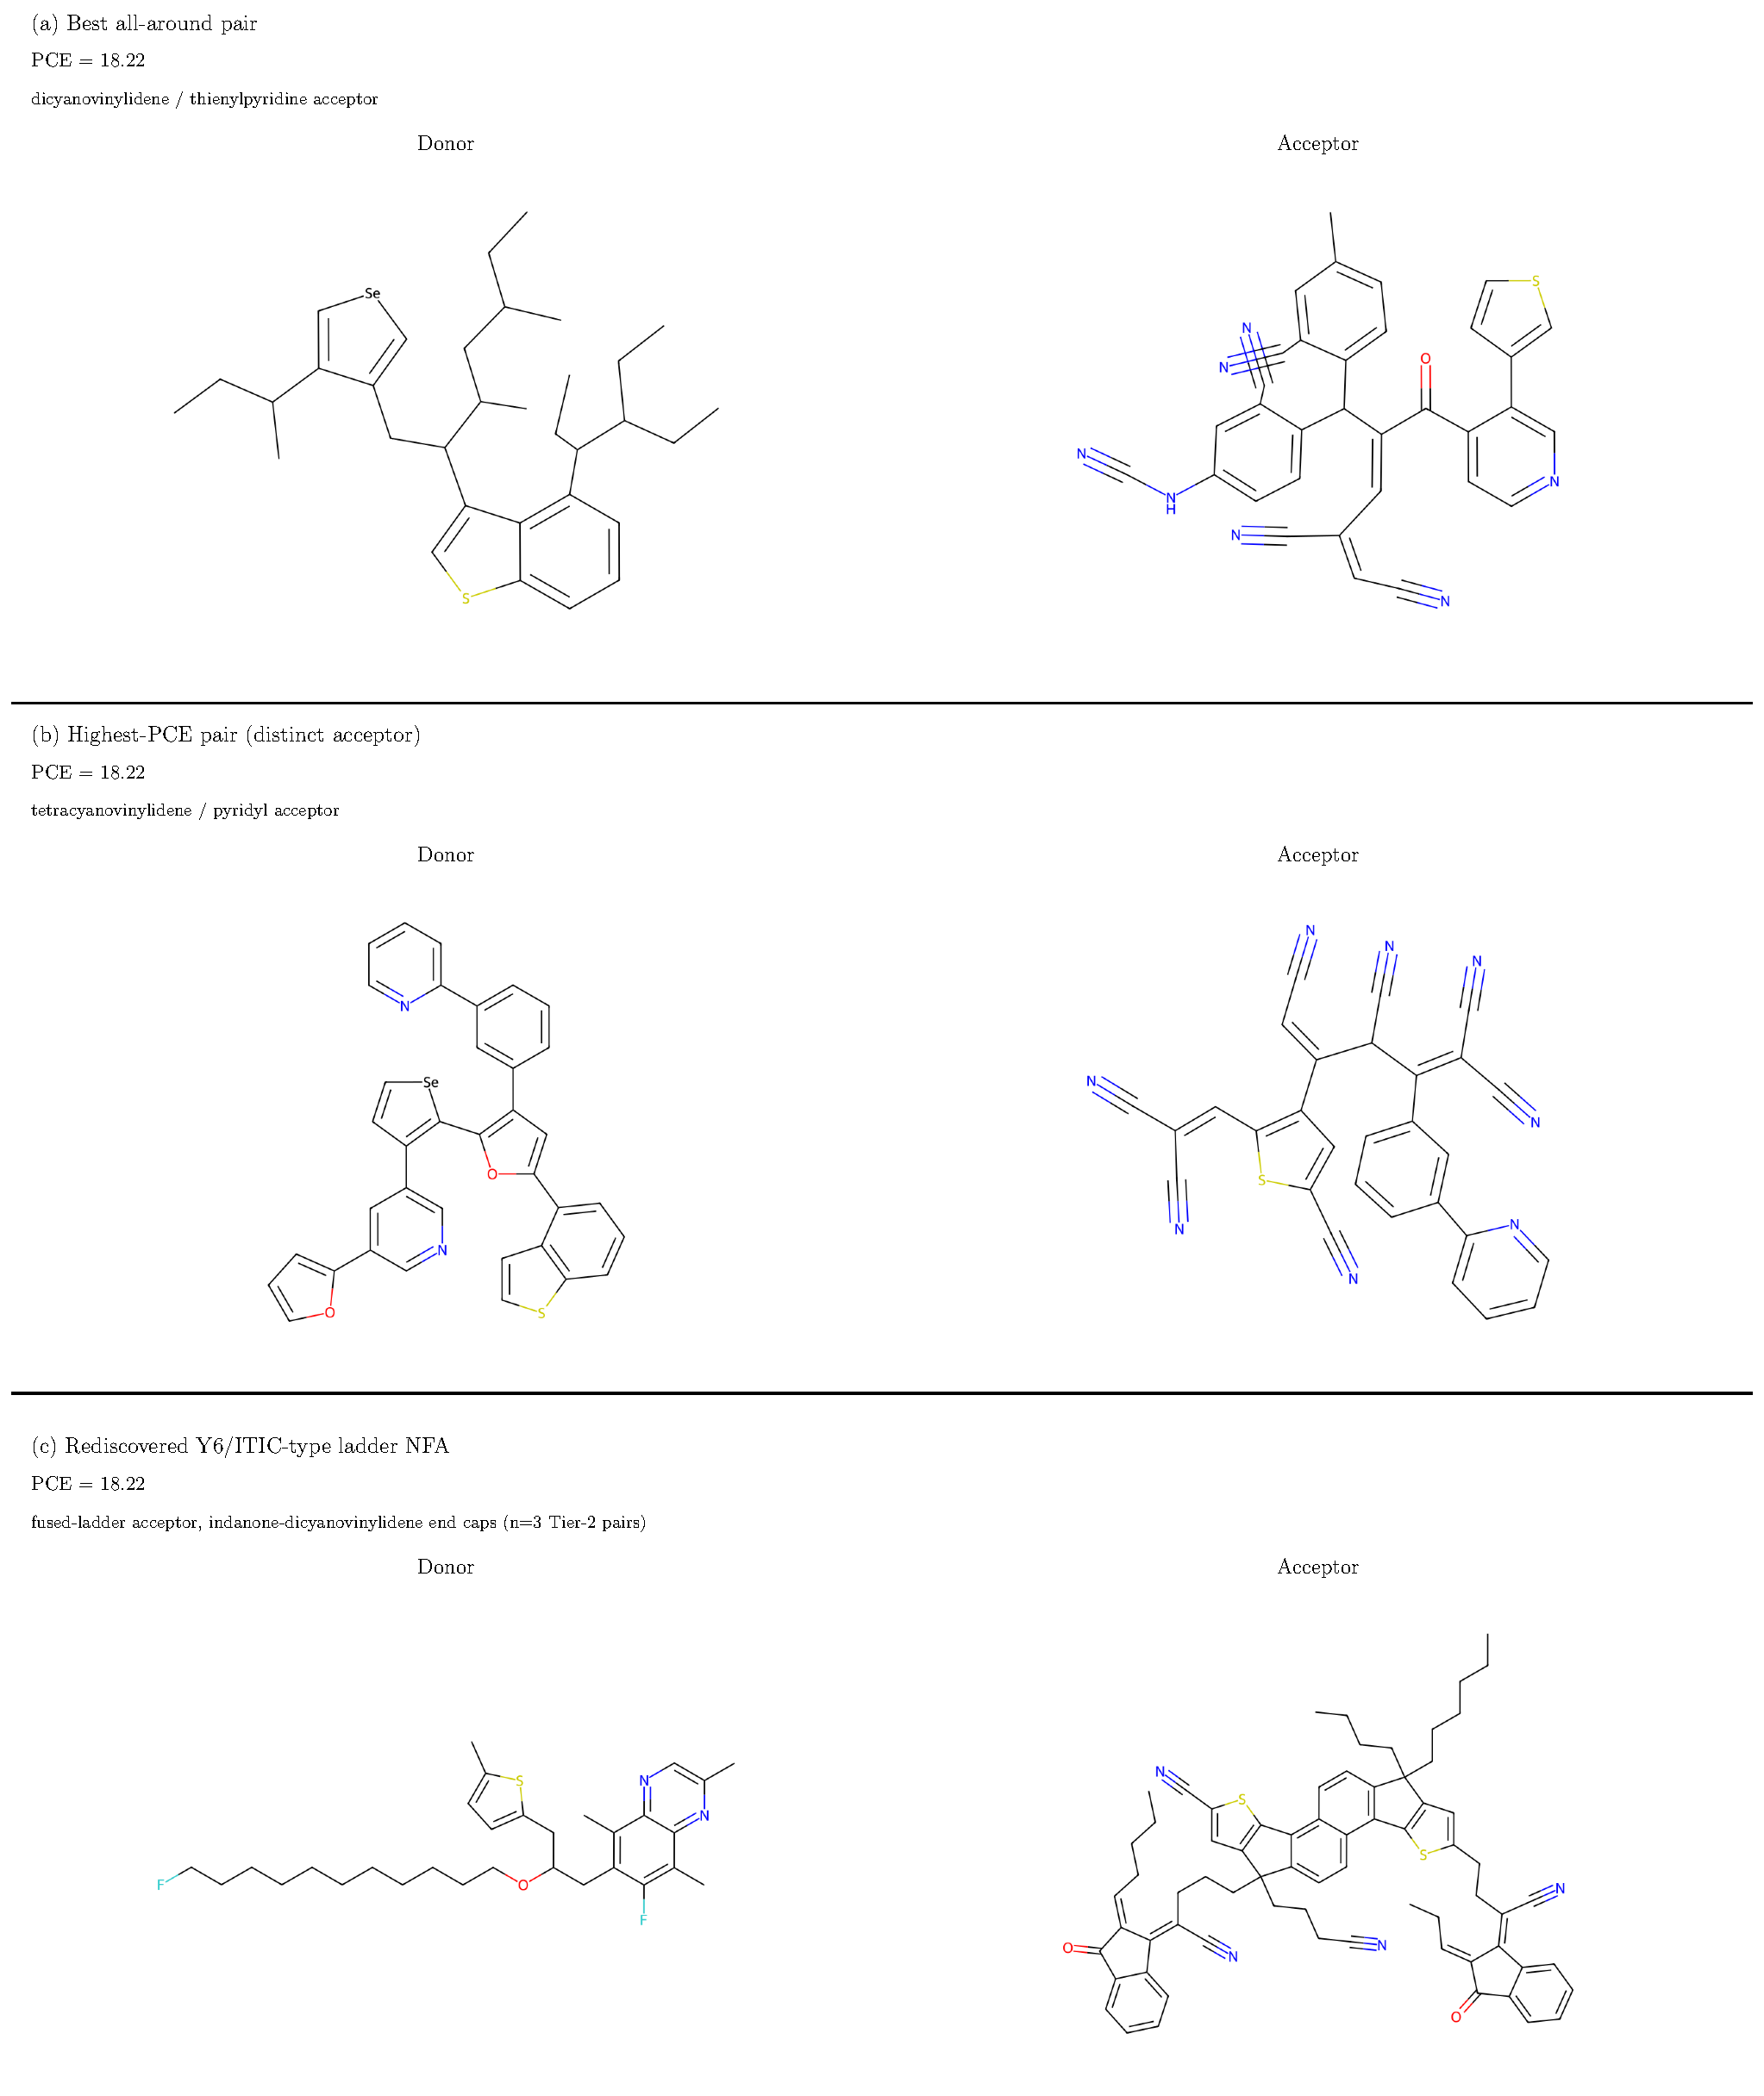
\includegraphics[width=15 cm]{figures/tier2_representative_pair.pdf}
\caption{Representative prioritized Tier-2 donor--acceptor pairs. (a) Highest-scoring all-round pair built on the most frequently recurring Tier-2 acceptor. (b) Chemically distinct pair with the maximum predicted PCE. (c) Fused-ladder NFA with a Y6/ITIC-type architecture and indanone--dicyanovinylidene end groups. Predicted values are screening-surrogate estimates for prioritization and not measured device efficiencies.}
\label{fig:tier2_representative_pair}
\end{figure}

Donor and acceptor recurrence nevertheless differ markedly within the shortlist. The ten most frequently occurring donors collectively account for only 5.9\% of the 2{,}832 Tier-2 pairs, with no donor appearing in more than 35 pairs. In contrast, the ten most frequent acceptors account for 48.1\% of the shortlist, and the most recurrent acceptor occurs in 172 pairs (Figure~S3). Tier-2 performance is thus distributed across a broad donor population but concentrated around a smaller set of high-scoring acceptor building blocks. This asymmetry identifies the recurring acceptor structures as particularly relevant targets for detailed structural and synthetic assessment.

The predicted frontier-orbital offsets were internally consistent with donor--acceptor pairing throughout the Tier-2 set. In all 2{,}832 pairs, the donor LUMO was higher than the acceptor LUMO, corresponding to a mean acceptor-referenced offset of $-1.51 \pm 0.27$ eV; the donor HOMO was likewise shallower than the acceptor HOMO, with a mean offset of $-0.78 \pm 0.15$ eV. Although these are screening-level estimates rather than DFT-computed or experimentally verified quantities, their consistent directionality indicates that the tiered filter did not retain pairs with inverted or degenerate predicted frontier-orbital alignment.

Figure~\ref{fig:tier2_representative_pair} illustrates three chemically distinct prioritized pairs. Panel~(a) shows the highest-scoring all-round pair, combining the most recurrent Tier-2 acceptor---a dicyanovinylidene/thienylpyridine push--pull chromophore present in 172 pairs---with its highest-scoring donor (PCE = 18.22\%, \jsc\ = 27.7 mA cm$^{-2}$, FF = 0.785, \voc\ = 0.862 V, and \Eloss\ = 0.54 eV). Panel~(b) shows a chemically distinct pair with the same maximum predicted PCE, based on a tetracyanovinylidene/pyridyl acceptor and a furan--thiophene--selenophene--benzothiophene--pyridine donor framework. Panel~(c) shows a generated fused-ladder NFA architecture related to Y6/ITIC-type systems, with an indacenodithiophene-like core and indanone--dicyanovinylidene end groups. This acceptor occurs in three Tier-2 pairs and reaches a predicted PCE of 18.22\% with its highest-ranked donor partner. Overall, 192 Tier-2 pairs attain the maximum predicted PCE, distributed across 15 distinct acceptors; the upper tail is therefore not attributable to a single acceptor structure. As throughout this work, these values are screening-surrogate estimates for prioritization and not claims of realized device performance.

\subsection{Energy Loss and Photovoltaic Performance}
The energy-loss parameter, $E_{\mathrm{loss}} = E_{\mathrm{opt}} - qV_{\mathrm{oc}}$, provides a physically meaningful measure of the energetic deficit between the optical excitation energy and the open-circuit voltage of a photovoltaic device. Lower \Eloss\ generally corresponds to more effective conversion of the available excitation energy into electrical output. Because an experimentally realizable photovoltaic device necessarily exhibits radiative and non-radiative voltage losses, we adopted approximately 0.25 eV as a physically meaningful lower bound for \Eloss, consistent with detailed-balance considerations \cite{benduhn}. In the 300-member reference dataset, 46 entries yield \Eloss\ $<$ 0.25 eV and are therefore considered physically inconsistent with this constraint. These cases arise from the approximate frontier-orbital treatment used to estimate \voc, which does not explicitly ensure that the predicted voltage remains below the optical gap. Accordingly, these entries are excluded from the quantitative analysis of the \Eloss--PCE relationship rather than being interpreted as physically meaningful low-loss devices.

The reference molecules that satisfy the physical energy-loss criterion span a broad range of photovoltaic performance, with \Eloss\ values ranging from approximately 0.25 to 1.3 eV and PCE values ranging from near 0 to above 18\%. The majority of experimentally relevant compounds are concentrated between approximately 0.4 and 0.9 eV in \Eloss, although several higher-efficiency examples occur at lower energy loss. The excluded entries occupy the unphysical region below 0.25 eV and span a wide range of apparent PCE values; their inclusion would therefore obscure the physically relevant relationship by introducing estimates based on an overestimated \voc.

\begin{figure}[!htb]
\centering
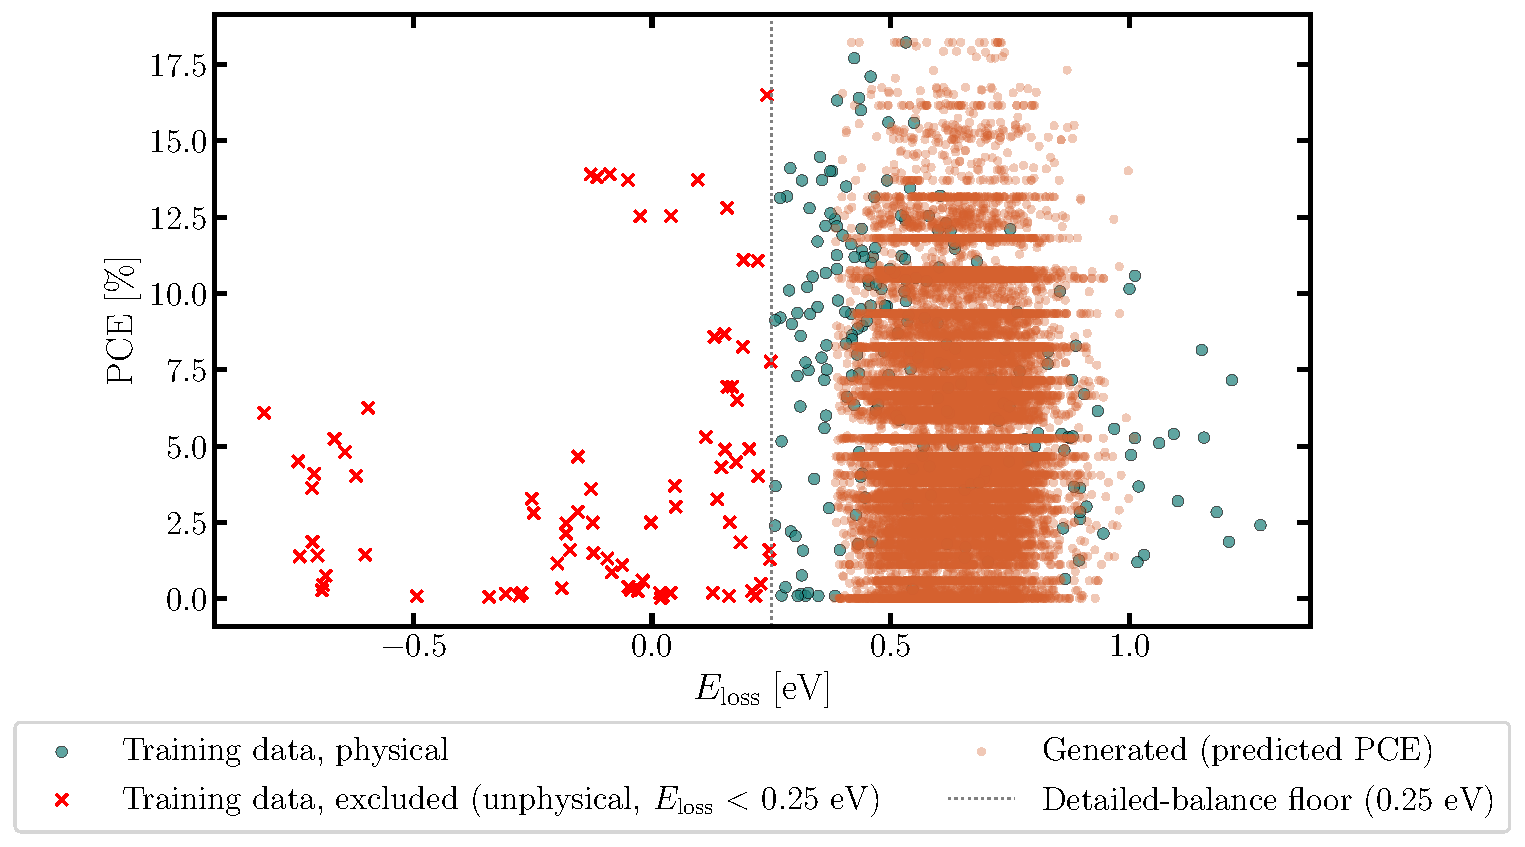
\includegraphics[width=12 cm]{figures/eloss_vs_pce_corrected.pdf}
\caption{Relationship between energy loss (\Eloss) and PCE for the reference data and generated donor--acceptor pairs. Reference entries below the physically credible energy-loss threshold of 0.25 eV are indicated separately. Generated-pair values are based on data-driven screening estimates and are intended for relative candidate prioritization.}
\label{fig:eloss_vs_pce_corrected}
\end{figure}

For the generated molecular pairs, the predicted distribution is concentrated predominantly within \Eloss\ $\approx$ 0.4--0.9 eV, overlapping the central region of the reference distribution. The corresponding PCE values are largely distributed between 0 and 8\%, with a progressively smaller population extending to higher efficiencies. The generated library nevertheless contains a distinct upper tail with predicted PCE values of approximately 17--18\%(Figure~\ref{fig:eloss_vs_pce_corrected}). This tail identifies regions of the generated chemical space that warrant closer assessment, but the predictions remain screening-level estimates and should not be interpreted as experimentally realized device efficiencies \cite{recorddevice}.

The mean predicted PCE of the generated population was 5.87\%, indicating that most candidates occupy a moderate-efficiency regime. Nevertheless, the coexistence of this broad central population with a smaller upper tail suggests that the workflow explores a wider range of predicted photovoltaic behavior than a narrow reproduction of the reference distribution. The low density of candidates jointly combining high predicted PCE and low \Eloss\ also highlights the inherent difficulty of enriching the generated chemical space toward this target region.

Taken together, these results indicate that the generated molecular pairs occupy a chemically and energetically plausible screening domain while retaining a limited population of candidates with jointly favorable predicted energy-loss and efficiency values. To identify focused candidates for experimental or higher-fidelity computational follow-up, we applied a joint sweet-spot criterion to the Tier-2 shortlist: \Eloss\ $\leq$ 0.55 eV and PCE $\geq$ 17.0\%. Of the 2{,}832 Tier-2 pairs, 33 (1.17\%) satisfy both conditions (Figure~S4), confirming that this combination remains rare even after tiered prioritization. {\com These pairs contain 33 distinct donors but only three distinct acceptors; one tricyanovinylidene/thienylpyridine-type acceptor, also identified as the most recurrent Tier-2 acceptor in Section~\ref{sec:tier2composition}, occurs in 28 of the 33 pairs (84.8\%).}

The highest-ranked sweet-spot pair combines this recurrent acceptor with a thiophene- or selenophene-substituted alkylated donor and has predicted PCE = 18.22\% and \Eloss\ = 0.54 eV. A chemically distinct pair based on the second most favorable acceptor motif reaches the same predicted PCE at \Eloss\ = 0.53 eV, albeit with a lower predicted fill factor (FF = 0.61 versus 0.79). These pairs are proposed as prioritized starting points for follow-up assessment rather than as validated device compositions.

\subsection{Overview of Molecular-Library Characteristics}
The generated molecular libraries combine substantial chemical-space coverage, structural diversity, and favorable computational indicators of synthetic accessibility, while providing a broad pool of candidates for subsequent device-level screening. The workflow therefore enables systematic exploration beyond the immediate reference chemical space and identifies a tractable subset of donor and acceptor structures for experimental investigation. At the same time, validation of the device-property surrogate demonstrates that its predictive reliability is target-dependent, with particularly limited quantitative accuracy for FF and \voc. Accordingly, the resulting device-property estimates are most appropriately used as relative ranking and prioritization criteria rather than as absolute predictions of experimentally realized device performance. The key quantitative outcomes of the workflow are summarized in Table S1.

\section{Conclusions}
We presented a synthesizability-aware hybrid molecular generation and screening workflow to expand the chemical space of OPV donors and NFAs. Twelve complementary proposal and augmentation routes generated class-specific molecular libraries that, after canonicalization, deduplication, and adaptive novelty filtering, yielded 52{,}995 unique donor candidates and 53{,}719 unique acceptor candidates. The low mean nearest-neighbor similarities and high internal and Bemis--Murcko scaffold diversity confirm that the retained libraries extend meaningfully beyond the reference chemical space while preserving a chemically interpretable relationship to the OPV training domain.

Synthetic practicality was assessed using \texttt{SAScore}, \texttt{RAscore}, and a TANGO-inspired building-block compatibility heuristic. Most of the generated molecules satisfied the combined accessibility screen (85.0\% of donors and 99.3\% of acceptors), and 76.5\% of the shortlisted structures were classified as route-findable using the available retrosynthetic backend. These outcomes provide useful comparative evidence of synthetic plausibility but do not establish experimentally executable routes; formal confirmation requires independent retrosynthetic analysis.

Pairing the filtered libraries produced 11{,}988{,}459 donor--acceptor combinations, of which 2{,}832 Tier-2 pairs jointly satisfied the chosen performance and compatibility criteria. The shortlisted pairs predominantly occupied a physically plausible energy-loss region and included a small high-performance tail with predicted PCE values approaching 18\%. Structure-disjoint validation showed weak-to-moderate transferability for PCE and \jsc, and unreliable quantitative accuracy for FF and \voc. The surrogate should therefore be used strictly for ranking and triage, with predictions interpreted as prioritization signals rather than as claims of realized device performance. The workflow provides a practical and chemically interpretable starting point for identifying OPV donor--acceptor candidates warranting experimental or higher-fidelity computational follow-up.


\section{Acknowledgements}
The authors gratefully acknowledge the Indian Institute of Technology Gandhinagar, India, for providing research facilities and financial support. We thank PARAM Ananta for computational resources. A.M. is grateful to the B. S. Gelot Chair, IIT Gandhinagar,
for the support.

\section{Supporting Information}
The Supporting Information contains additional computational details, the train--train split-half baseline analysis for the fingerprint-space Fréchet distance (Figure S1), the distributions of the most frequent Bemis--Murcko scaffolds among the unique donor and acceptor molecules in the Tier-2 shortlist (Figure S2), the recurrence of the ten most frequently occurring donor and acceptor building blocks within the Tier-2 shortlist (Figure S3), and the predicted energy-loss--PCE sweet-spot analysis for the Tier-2 pairs, highlighting candidates jointly satisfying $E_{\mathrm{loss}}\leq0.55$~eV, $\mathrm{PCE}\geq17.0\%$ (Figure S4), and a consolidated summary of molecular-library and validation metrics (Table~S1).


\section*{Author Contributions}
BD and AM conceived the problem. BD conducted all the simulations. BD and AM analyzed the results and prepared the draft.

\section*{Conflicts of interest}
There are no conflicts to declare.

\section*{Data Availability Statement} 
The data that support the findings of this study are available from the corresponding authors upon reasonable request.

\clearpage

\bibliographystyle{achemso}
\bibliography{references}

\vspace{1em}

% \begin{tcolorbox}[colframe=black, colback=white, fonttitle=\bfseries, title={\centering ToC Graphic}]
% \centering
% \includegraphics[width=0.5\textwidth]{figures/dyad_ToC.pdf}
% \end{tcolorbox}

\end{document}